%\documentclass[english,12pt]{article}
\documentclass[english,10pt]{article}
\usepackage[T1]{fontenc}
\usepackage[latin9]{inputenc}
\usepackage{babel}
\usepackage[dvipsnames,usenames]{color}
\usepackage{listings}
\usepackage{float}
%\usepackage{setspace}
\usepackage{times}
\usepackage{paralist}
%\usepackage{amsmath,amssymb,amsfonts}
%\usepackage{subfig}
%\usepackage{graphics}
%\usepackage{graphicx}
%\usepackage{wrapfig}
%\usepackage[ruled,vlined]{algorithm2e}
%\usepackage{url}
\usepackage{pdfpages}
\lstset{basicstyle=\ttfamily\scriptsize,emph={},emphstyle={\underbar},numbers=none,escapeinside={(*@}{@*)}}

% Generic macros (nothing specific to this paper)

\usepackage{ifthen}
%
\newcommand{\TODO}[1]{ {\color{blue} \bf #1} }
\newcommand{\AWK}[1]{ {\color{red} \bf #1} }
\newcommand{\TODOFN}[1]{ \footnote{{\bf #1}} }
\newcommand{\DONE}[1]{}
\newcommand{\COMMENT}[1]{}
\newcommand{\ie}{i.e.}
\newcommand{\eg}{e.g.}
%%% references definition
\newcommand{\lemref}[1]{Lemma~\ref{Lm:#1}}
\newcommand{\figref}[1]{Fig.~\ref{Fi:#1}}
\newcommand{\defref}[1]{Definition~\ref{De:#1}}
\newcommand{\theref}[1]{Theorem~\ref{Th:#1}}
\newcommand{\tabref}[1]{Tab.~\ref{Ta:#1}}
\newcommand{\secref}[1]{Section~\ref{Se:#1}}
\newcommand{\secrefs}[2]{Sections~\ref{Se:#1}-\ref{Se:#2}}
\newcommand{\ssecref}[1]{Sec.~\ref{Se:#1}}
%\newcommand{\subref}[1]{Subsection~\ref{Sub:#1}}
\newcommand{\appref}[1]{Appendix~\ref{Se:#1}}
\newcommand{\exref}[1]{Example~\ref{Ex:#1}}
\newcommand{\algref}[1]{Algorithm~\ref{Alg:#1}}
\newcommand{\lnref}[1]{line~\ref{Ln:#1}}
\newcommand{\lemlabel}[1]{\label{Lm:#1}}
\newcommand{\figlabel}[1]{\label{Fi:#1}}
\newcommand{\deflabel}[1]{\label{De:#1}}
\newcommand{\thelabel}[1]{\label{Th:#1}}
\newcommand{\tablabel}[1]{\label{Ta:#1}}
\newcommand{\seclabel}[1]{\label{Se:#1}}
\newcommand{\sseclabel}[1]{\label{Se:#1}}
%\newcommand{\sublabel}[1]{\label{Sub:#1}}
\newcommand{\applabel}[1]{\label{Se:#1}}
\newcommand{\exlabel}[1]{\label{Ex:#1}}
\newcommand{\alglabel}[1]{\label{Alg:#1}}
\newcommand{\lnlabel}[1]{\label{Ln:#1}}


\newtheorem{Example}{Example}
%\newtheorem{definition}{Definition}
%%\newtheorem{theorem}{Theorem}
%%% sectioning

\newcommand{\ignore}[1]{}

%% TO Allow writing the TR in the same source
\newboolean{TR}
\setboolean{TR}{false}
\ifthenelse{\boolean{TR}}{
\newcommand{\TrSelect}[2]{#1}
\newcommand{\TrOnly}[1]{#1}
\newcommand{\SubOnly}[1]{}
\newcommand{\TrOnlyInFootnote}[1]{#1}
\newcommand{\TrOnlyInTable}[1]{#1}}
{
\newcommand{\TrSelect}[2]{#2}
\newcommand{\TrOnly}[1]{}
\newcommand{\SubOnly}[1]{#1}
\newcommand{\TrOnlyInFootnote}[1]{}
\newcommand{\TrOnlyInTable}[1]{}}

%% General macros
\newcommand{\Set}[1]{\{ \; {#1} \; \}}
\newcommand{\vbar}{\; | \;}
\newcommand{\notIn}{\not\in}
\newcommand{\sizeof}[1]{|{#1}|}
%% \newcommand{\isDefined}{=_{def}}
\newcommand{\isDefined}{\triangleq}

\newcommand{\lt}{$<$}
\newcommand{\gt}{$>$}

%% tminus: "thin minus", with less space around it;
%% telem: "thin element"
\newcommand{\tminus}{\!\! - \!\!}
\newcommand{\telem}{\! \in \!}

%% stexttt: "small" texttt
\newcommand{\stexttt}[1]{{\small \texttt{#1}}}

\newcommand{\mathify}[1]{\mathord{\mbox{#1}}}
\newcommand{\italMathId}[1]{\mathify{\textit{\textrm{#1}}}}
\newcommand{\romanMathId}[1]{\mathify{\textup{\textrm{#1}}}}
\newcommand{\ttMathId}[1]{\mathify{\textup{\texttt{#1}}}}

\newcommand{\ttsub}[2]{${\ttMathId{#1}}_{#2}$}
\newcommand{\ttsup}[2]{${\ttMathId{#1}}^{#2}$}
\newcommand{\mttsub}[2]{{\ttMathId{#1}}_{#2}}
\newcommand{\twoarray[2]}{\begin{array}{l}  #1 \\ #2 \end{array}}
\newcommand{\subsubsubsection}[1]{\emph{#1}:}

%\newtheorem{theorem}{Theorem}[section]
%\newtheorem{lemma}[theorem]{Lemma}
%\newtheorem{proposition}[theorem]{Proposition}
%\newtheorem{corollary}[theorem]{Corollary}

%\newenvironment{proof}[1][Proof]{\begin{trivlist}\item[\hskip \labelsep {\bfseries #1}]}{\end{trivlist}}
%\newenvironment{definition}[1][Definition]{\begin{trivlist}\item[\hskip \labelsep {\bfseries #1}]}{\end{trivlist}}
%\newenvironment{example}[1][Example]{\begin{trivlist}\item[\hskip \labelsep {\bfseries #1}]}{\end{trivlist}}
%\newenvironment{remark}[1][Remark]{\begin{trivlist}\item[\hskip \labelsep {\bfseries #1}]}{\end{trivlist}}

%\newcommand{\qed}{\nobreak \ifvmode \relax \else
%      \ifdim\lastskip<1.5em \hskip-\lastskip
%      \hskip1.5em plus0em minus0.5em \fi \nobreak
%      \vrule height0.75em width0.5em depth0.25em\fi}

%% $Id: specificmacros.tex,v 1.22 2010/07/15 18:27:09 mkuper Exp $

\def\imagetop#1{\vtop{\null\hbox{#1}}}

\newcommand{\demonsmarker}{\textbf{DEMONS START HERE IF NOT EARLIER}}

\newcommand{\sectionette}[1]{\noindent \textit{#1}:}

\newtheorem{hypothesis}{Hypothesis}[section]
\newcommand{\hypref}[1]{Hypothesis~\ref{Hy:#1}}

\newcommand{\true}{T}
\newcommand{\false}{F}

\newcommand{\pline}[1]{#1}

\newcommand{\lnum}[1]{\textbf{#1}}
\newcommand{\reflnum}[1]{\texttt{#1}}

\newcommand{\term}[1]{\emph{#1}}

\newcommand{\authortext}[1]{{$\bullet$ \textsf{#1}}}
\newcommand{\hiddentext}[1]{}

\newenvironment{samePageBlock}{\par
\samepage
}{%
\par
\allowbreak }

\newcommand{\para}[1]{\vspace{3pt}\noindent\textbf{\textit{#1}}}
%\newcommand{\Lparagraph}[1]{\vspace{3pt}\noindent\textit{#1.}}
\newcommand{\Lparagraph}[1]{\vspace{-4pt}\paragraph{#1}}
%\newcommand{\LLparagraph}[1]{\noindent\textit{#1.}}
\newcommand{\tab}{\hspace*{2em}}

\newcommand{\correlate}{\bowtie}

\newcommand{\fvar}[2]{[#1\prec #2]}

\newcommand{\better}{\sqsubseteq}
\newcommand{\wbetter}{\unlhd}

\newcommand{\sep}{\ensuremath{\ \ | \ \ }}
\newcommand{\tool}{{\small \textsc{dizy}}}
\newcommand{\fpred}[2]{(#1\prec #2)}
\newcommand{\trans}[3]{#1\stackrel{#3}{\longrightarrow}#2}
\newcommand{\strans}[3]{#1\longrightarrow#2}
\newcommand{\mmname}{{\small \textsc{RLX}}}
\newcommand{\ebset}{\hat{E}}

\newcommand{\B}[1]{\langle{#1}\rangle}
\newcommand{\eqdef}{\buildrel \mbox{\tiny\rm def} \over =}

%%%%%%%%%%%%%%%%%%%%%%%%%%%%%%%%%%%%%%%%%%%%%%%%%%%%%
%% notation                                        %%
%%%%%%%%%%%%%%%%%%%%%%%%%%%%%%%%%%%%%%%%%%%%%%%%%%%%%

\newcommand{\optimal}{\ding{52}}
\newcommand{\success}{\ding{51}}
\newcommand{\failure}{\ding{55}}

%%%%%%%%%%%%%%%%%%%%%%%%%%%%%%%%%%%%%%%%%%%%%%%%%%%%%
%% Abstraction                                     %%
%%%%%%%%%%%%%%%%%%%%%%%%%%%%%%%%%%%%%%%%%%%%%%%%%%%%%

\newcommand{\eq}[1]{[#1]_{\alpha}}%{eq(#1)}

%%%%%%%%%%%%%%%%%%%%%%%%%%%%%%%%%%%%%%%%%%%%%%%%%%%%%
%% Terminology                                     %%
%%%%%%%%%%%%%%%%%%%%%%%%%%%%%%%%%%%%%%%%%%%%%%%%%%%%%
\newcommand{\scode}[1]{{\small \texttt{#1}}}
\newcommand{\sname}[1]{{\small \textsc{#1}}}

%%%%%%%%%%%%%%%%%%%%%%%%%%%%%%%%%%%%%%%%%%%%%%%%%%%%%
%% Actions and Traces                              %%
%%%%%%%%%%%%%%%%%%%%%%%%%%%%%%%%%%%%%%%%%%%%%%%%%%%%%

\newcommand{\interseq}[1]{{\small\texttt{#1}}}

%%%%%%%%%%%%%%%%%%%%%%%%%%%%%%%%%%%%%%%%%%%%%%%%%%%%%
%% Semantics                                       %%
%%%%%%%%%%%%%%%%%%%%%%%%%%%%%%%%%%%%%%%%%%%%%%%%%%%%%

\newcommand{\lsyn}{\lbrack\!\lbrack}
\newcommand{\rsyn}{\rbrack\!\rbrack}
\newcommand{\semp}[1]{\lsyn #1 \rsyn}
\newcommand{\asemp}[1]{\lsyn #1 \rsyn^{\sharp}}

\newcommand{\slen}[1]{|#1|}

\newcommand{\dpless}{<_{\sigma,p}}

\newcommand{\concat}{\cdot}

%% States
\newcommand{\States}{\Sigma}
\newcommand{\sStates}{\Sigma_s}
\newcommand{\pStates}{\Sigma_p}
\newcommand{\mStates}{\Sigma_M}

%% Transitions
\newcommand{\Transitions}{\mbox{{\it \Tau}}}
\newcommand{\pTrans}{\Tau_p}
\newcommand{\mTrans}{\Tau_M}


%% Sets of States
\newcommand{\Stuck}{\mbox{{\it Stuck}}}
\newcommand{\Doomed}{\mbox{{\it Doomed}}}
\newcommand{\Initial}{\mbox{{\it Init}}}


%% Program
\newcommand{\Labels}{\italMathId{Labs}}
\newcommand{\Statements}{\italMathId{Stmts}}
\newcommand{\SharedVar}{\italMathId{Shared}}
\newcommand{\LocalVar}{\italMathId{Local}}
\newcommand{\stmt}{\mbox{{\it stmt}}}
\newcommand{\Value}{\mbox{{\it Int}}}
\newcommand{\val}[2]{\semp{#1}(#2)}
\newcommand{\Reach}{\mbox{{\it Reach}}}

%% Relations
\newcommand{\patharrow}{\rightsquigarrow}

%% General
\newcommand{\valid}{\mbox{{\it valid}}}
%\newcommand{\implies}{\Rightarrow}
\newcommand{\wgamma}{\widehat{\gamma}}
\newcommand{\powerset}{\mathcal{P}}
\newcommand{\dominatedBy}{\mbox{{\it DominatedBy}}}
\newcommand{\Ideal}{\mbox{{\it Ideal}}}
%\newcommand{\Obs}{\mbox{{\it Obs}}}
\newcommand{\Op}{\mbox{{\it Op}}} %% operations
\renewcommand{\phi}{\varphi}


\newcommand{\atomic}[2]{{\footnotesize \texttt{[#1,#2]}}}

\newcommand{\atomicmath}[2]{[#1,#2]}

\newcommand{\scheduled}{\mbox{\textit{atomic}}}
\newcommand{\nodes}{\mbox{\textit{states}}}

\newcommand{\MA}{\mbox{\textit{MA}}}

\newcommand{\aeq}{\preceq_{\alpha}}

\newcommand{\Abs}{\Sigma^{\natural}_P}
\newcommand{\Traces}{\mbox{\scode{Traces}}}

\newcommand{\C}[1]{#1^\natural} % for all concrete symbols
\newcommand{\A}[1]{#1^\sharp} % for all abstract symbols
\newcommand{\PS}[1]{{2^{#1}}}
\newcommand{\StatesConc}{\C{C}}
\newcommand{\Formulas}{Formulas}
\newcommand{\Dom}{Dom}
\newcommand{\Below}{\sqsubseteq}
\newcommand{\violated}{Av}
\newcommand{\UStates}{\Upsilon}
\newcommand{\evalf}[2]{\llbracket #2 \rrbracket_{#1}}
\newcommand{\enf}[2]{E_{\fpred{#1}{#2}}}
\newcommand{\admits}[2]{#1\smile #2}
\newcommand{\nadmits}[2]{#1\not\smile #2}

\newcommand \abssem[1]{Abs\textsubscript{[1,#1]}}
\newcommand{\semref}[1]{Sem.~\ref{Fi:#1}}

%\newcommand{\SBa}{SB1}
\newcommand{\SBb}{RA}
\newcommand{\SBc}{PDA}
\newcommand{\SBd}{OA}

\newcommand{\NoPJ}{FD}
\newcommand{\PJ}{PD}

\newcommand{\PD}[1]{{#1}^\tau}


\begin{document}
\title{Research Proposal for Ph.D. Thesis:\\ \vspace{0.1in} \textsc{Differential Program Analysis}}
\author{Nimrod Partush\\
        Technion, Haifa \\ \\
        Supervisor: Dr. Eran Yahav\\}
\maketitle
\newpage
\mbox{}
\newpage
\tableofcontents
\newpage
\mbox{}
\newpage
\begin{abstract}
We address the problem of correlating closely related versions of a program.
\end{abstract}

\section{Introduction} \seclabel{Intro}

%% what are we trying to say?
% 1. computing semantic diff is important
% 2. computing semantic diff is hard
% 3. existing approaches for computing semantic diff suck
% 4. our approach is great
% 5. technically, we use the following ideas:
%    - correlating program
%    - correlating abstract domains

% TODO:
% - we should have a clear problem definition somewhere
% - what is so special about a patched program?

Computing semantic difference for characterizing change in behavior due to code modification can be invaluable for the process of software development. Every change to the code requires careful consideration of questions like (i) did the patch add/remove the desired functionality? (ii) does the patch affect other, \emph{unexpected}, behaviors? (iii) which regression tests need be run? which break and why?. Answering these often consume a considerable amount of the development time, especially in legacy code where the developer of the original developer is no longer present.

Semantic differencing and program equivalence is considered a fundamental problem in computer science, receiving much attention from classical work~\cite{} and recently it has been flagged as a goal for static analysis methods~\cite{}. The applications of semantic equivalence and differencing range from contract checking, patch integration debugging and regression test generation and pruning. Recent work ~\cite{} also show the security implications of semantic differencing for exploit generation.

\para{Existing Techniques}
Existing techniques mostly offer under-approximating solutions, the prominent of which is regression testing which provides very limited assurance as to whether the behavior changes correctly as tests usually cover a fraction of program behaviors. Furthermore, running regression on large systems requires integrating the changed module into the entire system which can consume time, especially considering the actual time of running the entire regression. Godlin and Strichman~\cite{GodlinStrichman09} rely on bounded model checking techniques to produce a (binary) result regarding (input-output) equivalence two closely related numerical programs. \TODO{Further work~\cite{KawaguchiLahiriRebelo10} define the notion of conditional equivalence but are unable to describe difference in loops}. Other techniques for describing difference
~\cite{DwyerElbaumPerson08,EnglerRamos12} which rely on
symbolic execution supply unsound results as they are limited by loops and
essentially cover a subset of program behavior. \TODO{mention classical work like \cite{Horwitz:PLDI90,Horwitz:TOPLAS89}}

We present an approach based on abstract program interpretation for a \textbf{sound}, succinct representation of changed program behaviors and proving equivalence. Our method focuses on abstracting relationships between variables, and therefore behaviors, in both versions allowing us to achieve a precise description of difference and prove equivalence while ignoring other program information which may encumber a traditional analysis but is less relevant in our setting\footnote[1]{Eran: you didn't like this sentence, i love it, i'm trying to say we abstract away numerical information etc. and focus on relationships, thus we have better results since we are not encumbered by this less relevant information}.

\para{Problem Definition}
We define the problem of program equivalence and difference as follows: Given a pair of programs $(P,P')$ which agree on the number and type of inputs, for every execution of $P$ that originate from an input $i$ and a matching execution of $P'$ that originates from the \textbf{same input $i$} we describe:
\begin{itemize}
\item Whether these executions agree on output i.e. exhibit the same behavior.
\item In case of difference in behavior, provide a description of difference.
\end{itemize}
We intentionally define the notion of input and output equivalence loosely as this allows a more flexible definition of difference.

As the number of executions is unbound, we require abstraction in order to soundly compute this result. Though the notion of difference is well defined in the concrete case, defining and soundly computing it under abstraction is challenging as:
\begin{itemize}
\item Differencing requires correlation of \emph{different program executions} meaning the abstraction must limit itself to capturing differences of same-input executions, which is problematic under trace abstraction.
\item Establishing equivalence under abstraction is challenging since equality under abstraction does not entail concrete equality.
\end{itemize}

\para{Correlating Program}
Abstracting relationships allows us to maintain focus on difference while
omitting (whenever necessary for scalability) parts of the behavior that does
not entail difference. In order to monitor these relationships we created a
\emph{correlating program} which captures the behavior of both the original
program and its patched version. Instead of designing a correlating semantics
that is capable of co-executing two programs, we chose to automatically
construct the correlating program such that we can benefit from the use of
standard analysis frameworks for analyzing the resulting program. Another
advantage of this new construct, is that you may apply other methods for
equivalence checking directly on it~\cite{EnglerRamos11} as the correlation
allows for a much more fine-grained equivalence checking (between local
variables and not only output).

\para{Correlating Abstraction}
Our abstraction holds data of both sets of variables, joined together and is
initialized to hold equality over all matched variables. This means we can
reflect relationships without necessarily knowing the actual value of a
variables (we can know that $x_{old} = x_{new}$ even though actual values are
unknown). We ran our analysis over the correlating program while updated the
domain to reflect program behavior. Since some updates may result in non-convex information (e.g. taking  a condition of the form $x \neq 0$ into account), our domain has to represent non-convex information, at least temporarily. We address this by working with a powerset domain of a convex representation with partitioning according to equivalence criteria to avoid exponential blowup. Our domain may over-approximate numerical information as long as equivalence between correlated variables is preserved.

\subsection{Main Contributions}
The main contributions of this paper are as follows:
\begin{itemize}
\item we present a method for abstract interpretation of a pair of programs $(P,P')$ for \emph{sound} semantic equivalence and differencing by abstracting direct relationships between $(P,P')$ variables in a partially disjunctive domain. We describe a partitioning technique for state reduction and scaling. We define a widening operator for abstracting unbound paths in our domain.
\item we phrase a new technique for syntactically interleaving a pair of programs $(P,P')$ for the creation of a \emph{correlating program} $P \bowtie P'$ which contains the semantics of both programs. We propose an analysis over the program for characterizing program equivalence and difference, based on the aforementioned abstraction, given the properties of the correlating program which aligns $(P,P')$ executions.
\item We have implemented our approach in a tool based on the LLVM compiler infrastructure and the APRON numerical abstract
    domain library, and evaluated it using over 50 patches from open-source software including GNU core utilities, Mozilla
    Firefox, and the Linux Kernel. Our evaluation shows that the tool often manages to establish equivalence, reports useful
    approximation of semantic differences when differences exists, and reports only a few false differences.
\end{itemize}



\section{Overview}\seclabel{Overview}

\begin{figure}
\centering
\begin{tabular}{ccc}
\begin{lstlisting}
int sign(int x) { 
  int sgn;
  if (x < 0)
    sgn = -1
  else 
    sgn = 1
 return sgn
}
(*@ \vspace{0.1in} @*)
\end{lstlisting}
&
&
\begin{lstlisting}
int sign'(int x) {
  int sgn;
  if (x < 0)
    sgn = -1
  else if (x==0)
    sgn = 0
  else 
    sgn = 1
 return sgn
}
\end{lstlisting}
\\
\end{tabular}
\caption{Two simple implementations of the \emph{sign} operation.}
\figlabel{SignExample}
\end{figure}


Consider the simple example program of~\figref{SignExample}, inspired by an example from~\cite{MauborgneRival07}. For this example, we would like to establish that the output of $sign$ and $sign'$ only differ in the case where $x=0$ and that the difference is $sgn = 1 \neq sgn' = 0$. An optimal characterization of behavior is as following:
\\
\begin{tabular}{l|l|l}
$x.x'$ constraints  & $sgn$             & $sgn'$
\\ \hline
$x < 0$             & $sgn \mapsto -1$  & $sgn' \mapsto -1$
\\ \hline
$x = 0$             & $sgn \mapsto 1$  & $sgn' \mapsto 0$
\\ \hline
$x > 0$             & $sgn \mapsto 1$  & $sgn' \mapsto 1$
\end{tabular}
\\

As a first naive attempt to achieve such a description, one could try to analyze each version of the program separately and compare the (abstract) results. However, this is clearly unsound, as equivalence under abstraction does not entail concrete equivalence. For example, using a interval analysis~\cite{CousotHalbwachs78} would yield that in both programs the value of \scode{sgn} ranges in the same interval $[-1,1]$, missing the fact that $sign$ never returns the value $0$.

%\begin{wrapfigure}{r}{0cm}
%\imagetop{
%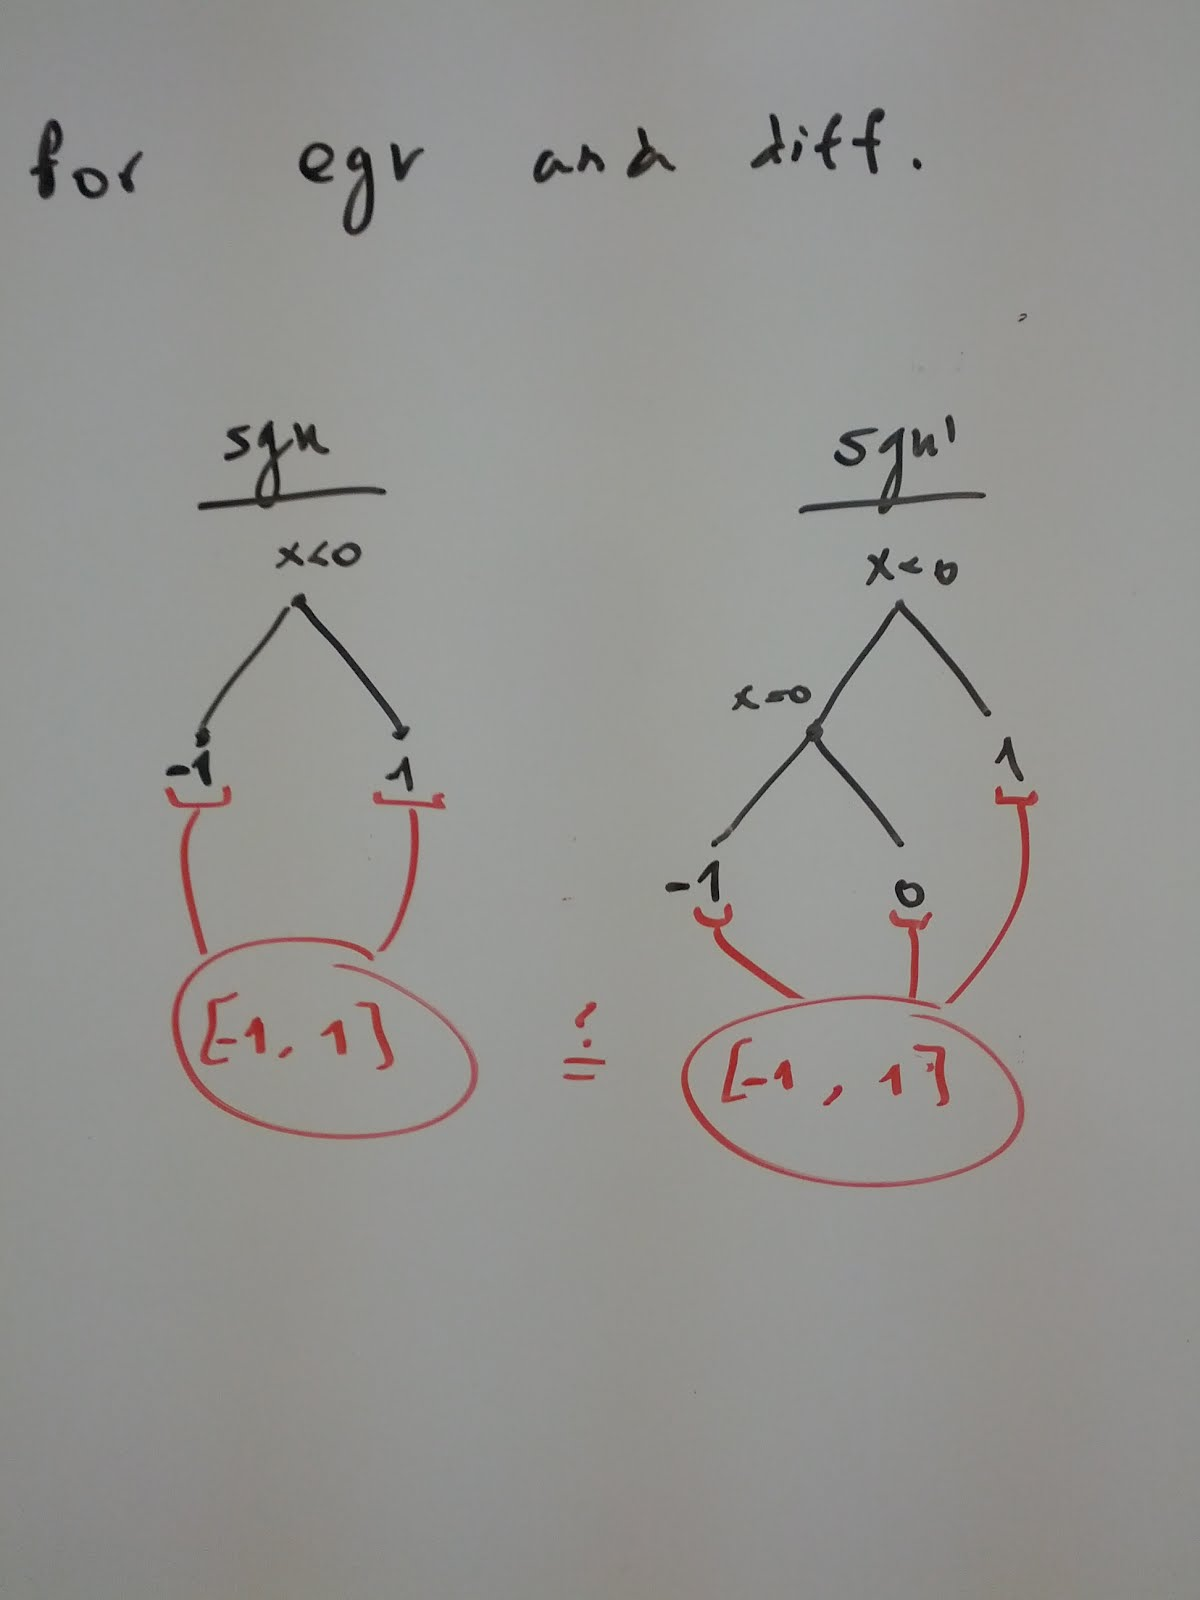
\includegraphics[scale=0.15,clip=true,trim = 125pt 400pt 125pt 350pt]{figures/sign-interval.jpg}
%}
%\caption{Interval analysis unsound comparison for $sign$ and $sign'$}\figlabel{SignInterval}
%\end{wrapfigure}

Furthermore, this result entirely ignores how $x$ affects the value of $sgn$ thus we would have no means to differentiate correctly, by input (e.g. we will get the same result for the $-1 * sign$ function).

To establish equivalence under abstraction, we need to abstract relationships between the values of variables in $sign$ and $sign'$ under the assumption of equivalence of input. Specifically, we need to track the relationship between the values of \scode{sgn} in both versions and see whether we can establish their equivalence. Tracking relationships dictates performing a \emph{joint analysis} that employs a \emph{correlating abstraction} allowing us to bind variables of both programs in one abstract state.

A correlating-oriented abstraction is well suited for proving equivalence as it allows focusing on relationships between versions of variables while abstracting away other (numerical) information allowing us to scale better. Most importantly, such an abstraction guarantees that equivalence will be reported soundly: as in a separate analysis we abstracted $\langle sgn \mapsto -1 \rangle$ and $\langle sgn \mapsto 1 \rangle$ towards an interval $\langle sgn \mapsto [-1,1] \rangle$, and again for $sgn'$ values, separately, which cannot assure equivalence (and in fact shouldn't). We instead use correlating states: $s_1 = \langle sgn = sgn' \mapsto -1 \rangle$ and $s_2 = \langle sgn = sgn' \mapsto 1 \rangle$, which allow us to abstract as such $s_1 \sqcup s_2 = \langle sgn = sgn', sgn \mapsto [-1,1] \rangle$ so equivalence can be soundly assured.

%If we instead use disjunctive completion powerset domain~\cite{TODO} where the abstract state is a set of convex sub-states, and no merge is ever performed, this would yield a precise result that may be used for equivalence checking and differencing.  For instance, using such domain for $sign$ would yield: $\langle x < 0, sgn = -1 \rangle \vee \langle x \geq 0, sgn = 1 \rangle$ and for $sign'$: $\langle x < 0, sgn = -1 \rangle \vee \langle x > 0, sgn = 1 \rangle \vee \langle x = 0, sgn = 0 \rangle$. Further refining $sign$'s abstraction and splitting the $\langle x \geq 0, sgn = 1 \rangle$ constraint to $\langle x > 0, sgn = 1 \rangle \vee \langle x = 0, sgn = 0 \rangle$ would allow perfectly aligning the input constraints to produce the difference of $x=0,sgn=1,sgn'=0$ as depicted in \figref{SignComplete}.
%\begin{wrapfigure}{r}{0cm}
%\imagetop{
%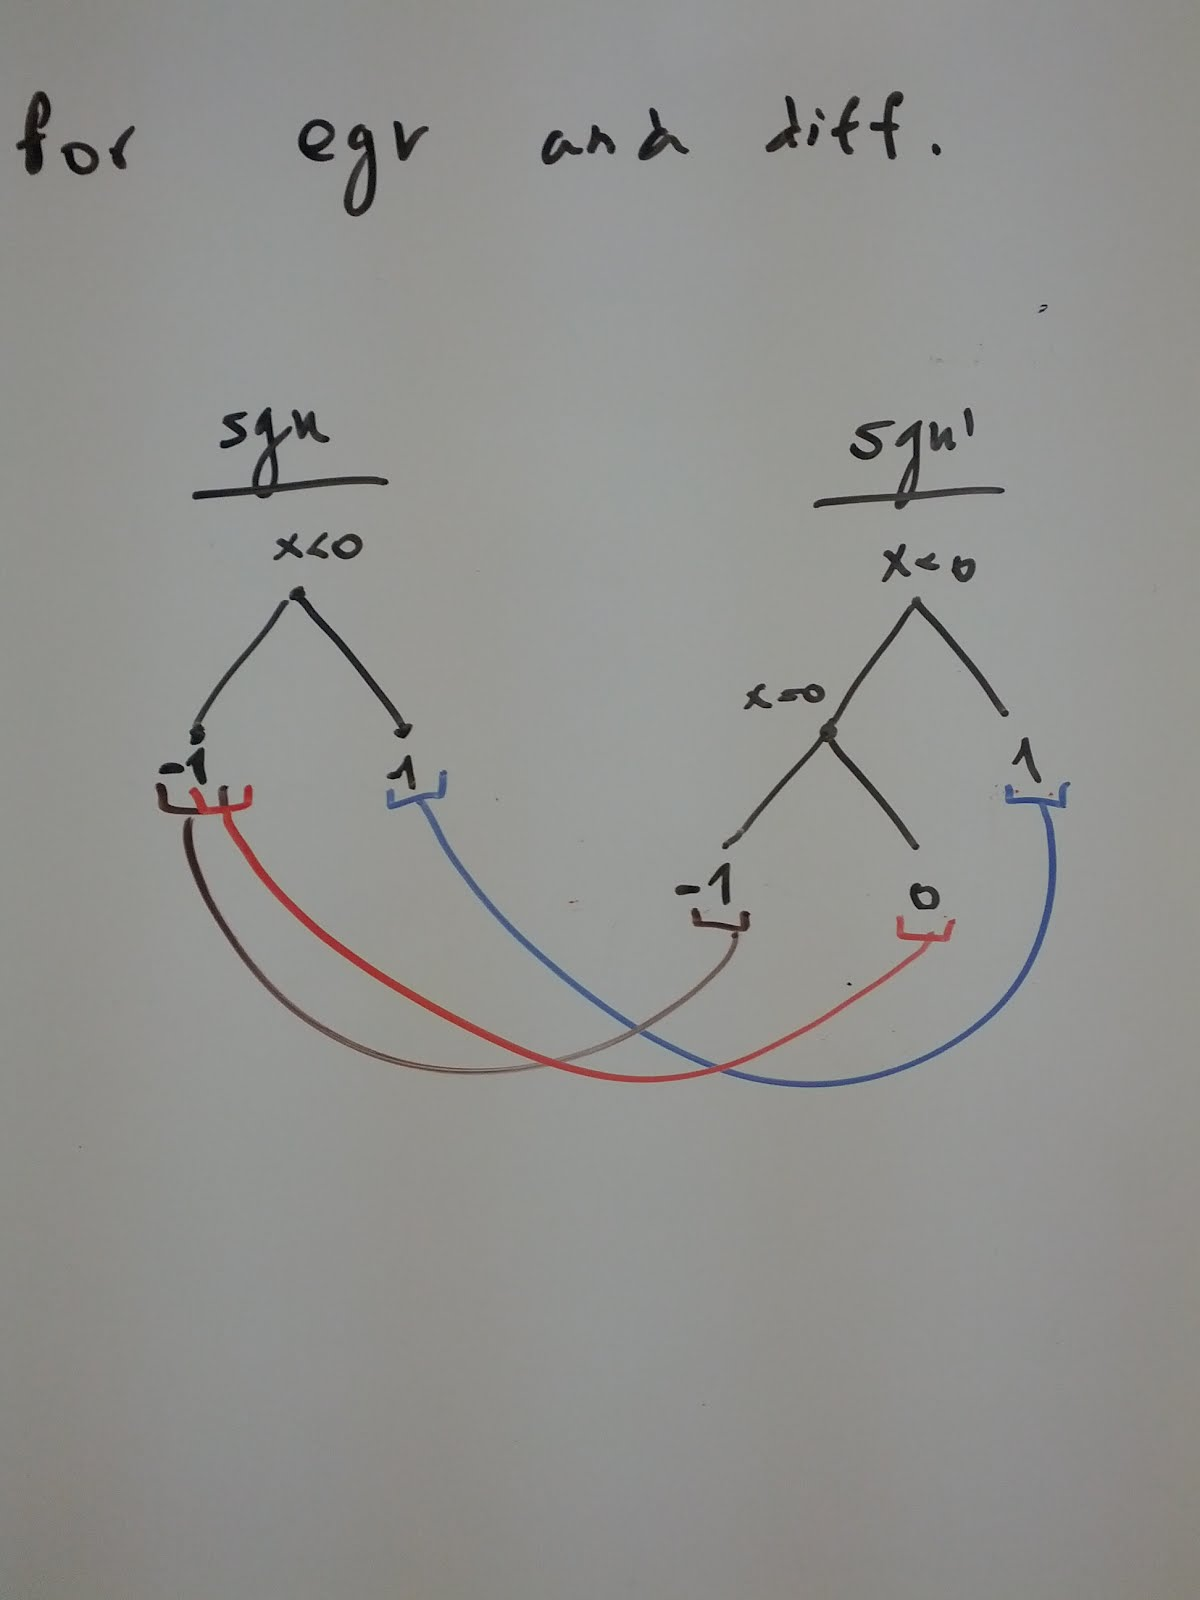
\includegraphics[scale=0.15,clip=true,trim = 125pt 450pt 100pt 350pt]{figures/sign-complete.jpg}
%}
%\caption{Complete disjunction analysis sound comparison for $sign$ and $sign'$}\figlabel{SignComplete}
%\end{wrapfigure}

We present an abstraction over dual program state, thats able to correlate paths that originate from the same input as well as produce a characterization of equivalence and difference which reflects change in behavior precisely. For example, we produce the following constraints for $sign$ and $sign'$:
\\
\begin{tabular}{ccc}
\hspace{1cm} $\sigma_{\times}^1 = \{x = x' < 0, sgn = sgn' \mapsto -1\}$
\\
\hspace{1cm} $\sigma_{\times}^2 = \{x = x' = 0, sgn \mapsto 1, sgn' \mapsto -1\}$
\\
\hspace{1cm} $\sigma_{\times}^3 = \{x = x' > 0, sgn = sgn' \mapsto 1\}$
\\
\end{tabular}
\\

To arrive at this result, we used an initial setting which abstracted the dual program state by analyzing both programs sequentially ($P;P'$), while updating the shared state with data regarding both sets of variables, while allowing a complete disjunction over all paths. In order to correlate paths by input and arrive at a precise disjunction, the analysis initially assumes input equivalence $\vec{i} = \vec{i'}$.

In this setting, as we advance through the analysis of $P$, we will accumulate the disjunction of all possible path constraints in its final state (this is similar to trace partitioning~\cite{MauborgneRival07}). At this point, as we continue to analyze $P'$, each disjunct representing a path in $P$ will be further conjuncted with all of $P'$ paths. This will produce a precise disjunction for differencing as each path in $P$ will be split and conjuncted with all of $P'$ paths, while avoiding considering conjunctions that disagree on input due to our input equivalence assumption. An illustration of the joint analysis for the $sign$ example can be seen in \figref{SignAnalysis1} including markings for feasible and infeasible paths.

%In some cases, it would have been sufficient to use alternative domains that are capable of representing richer information, such as interval polyhedra~\cite{CMWC:SAS09}, or other numerical domains that can represent non-convex information (e.g., \cite{TODO}). The recent donut domain~\cite{GIBMG:VMCAI12} may be of particular interest for this purpose. However, the general principle of having to preserve correlating information even when information about the values is abstracted away, holds in all of these cases.

%\begin{figure}
%\imagetop{
%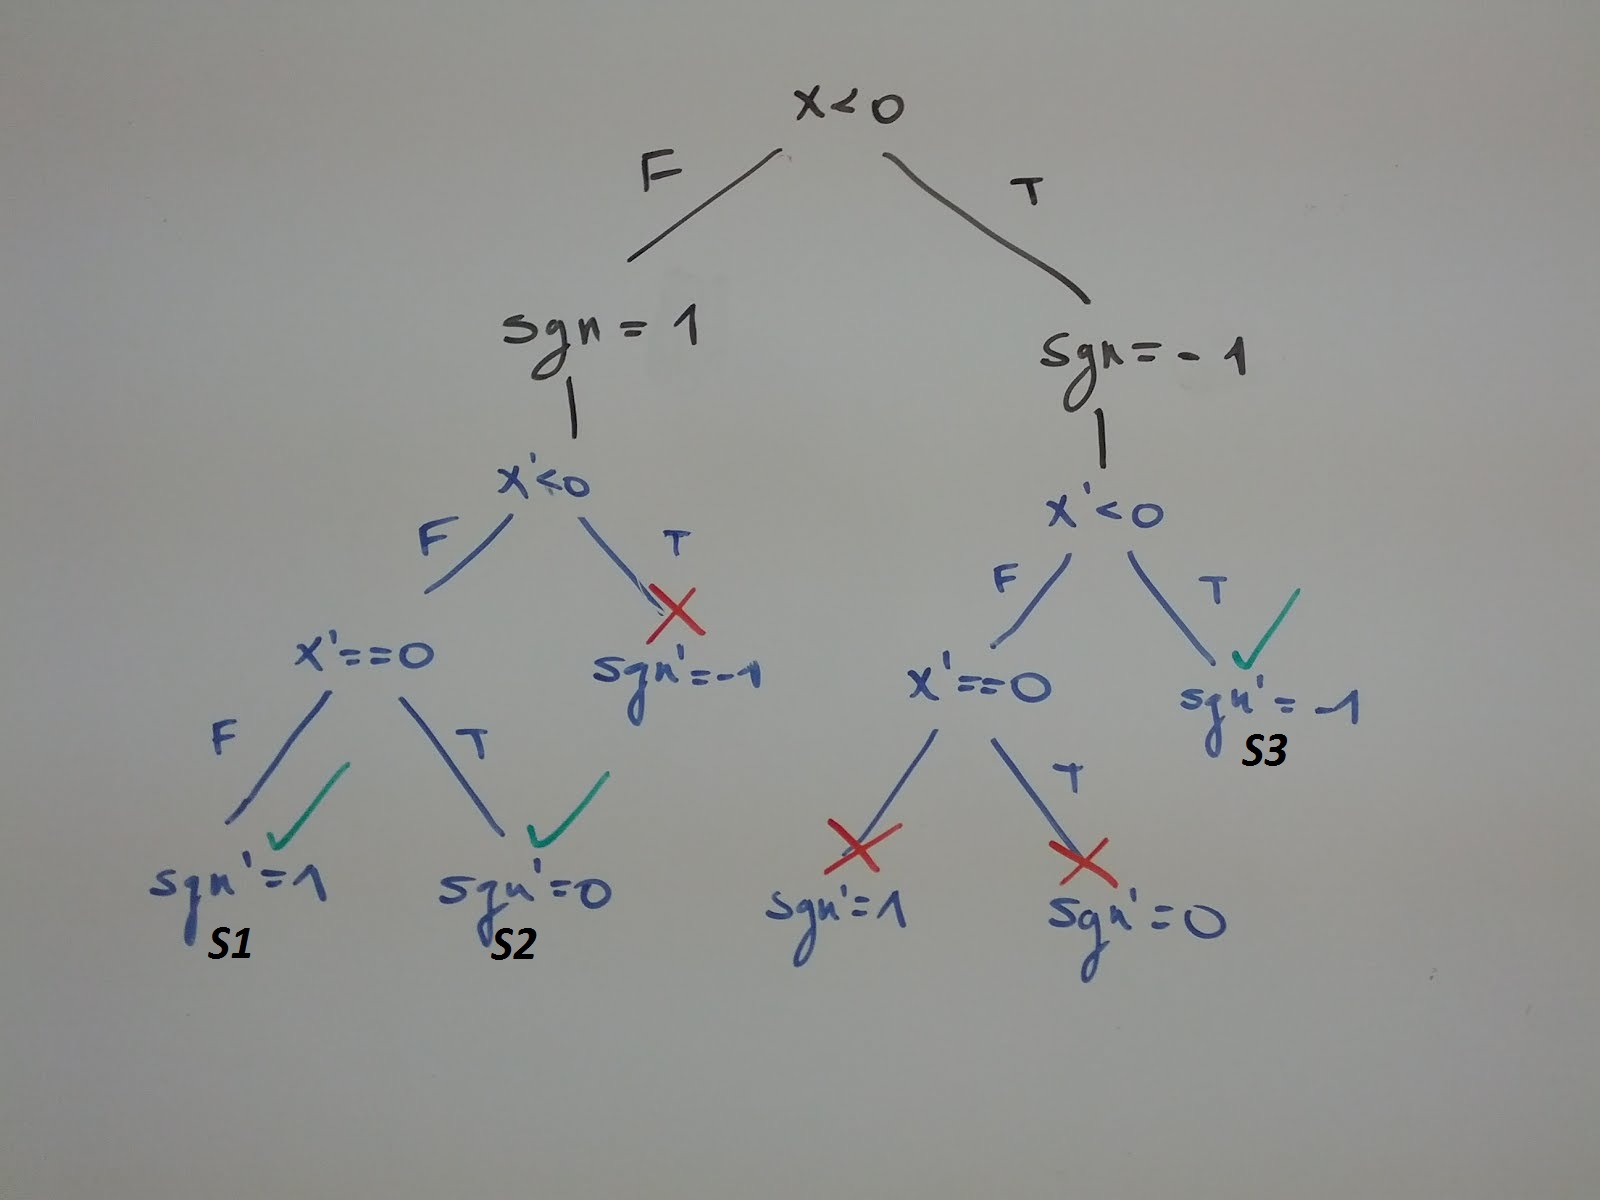
\includegraphics[scale=0.28,clip=true,trim = 50pt 100pt 100pt 0pt]{figures/sign-analysis1.jpg}
%}
%\caption{Joint $sign;sign'$ analysis}\figlabel{SignAnalysis1}
%\end{figure}

\begin{figure}
\centering
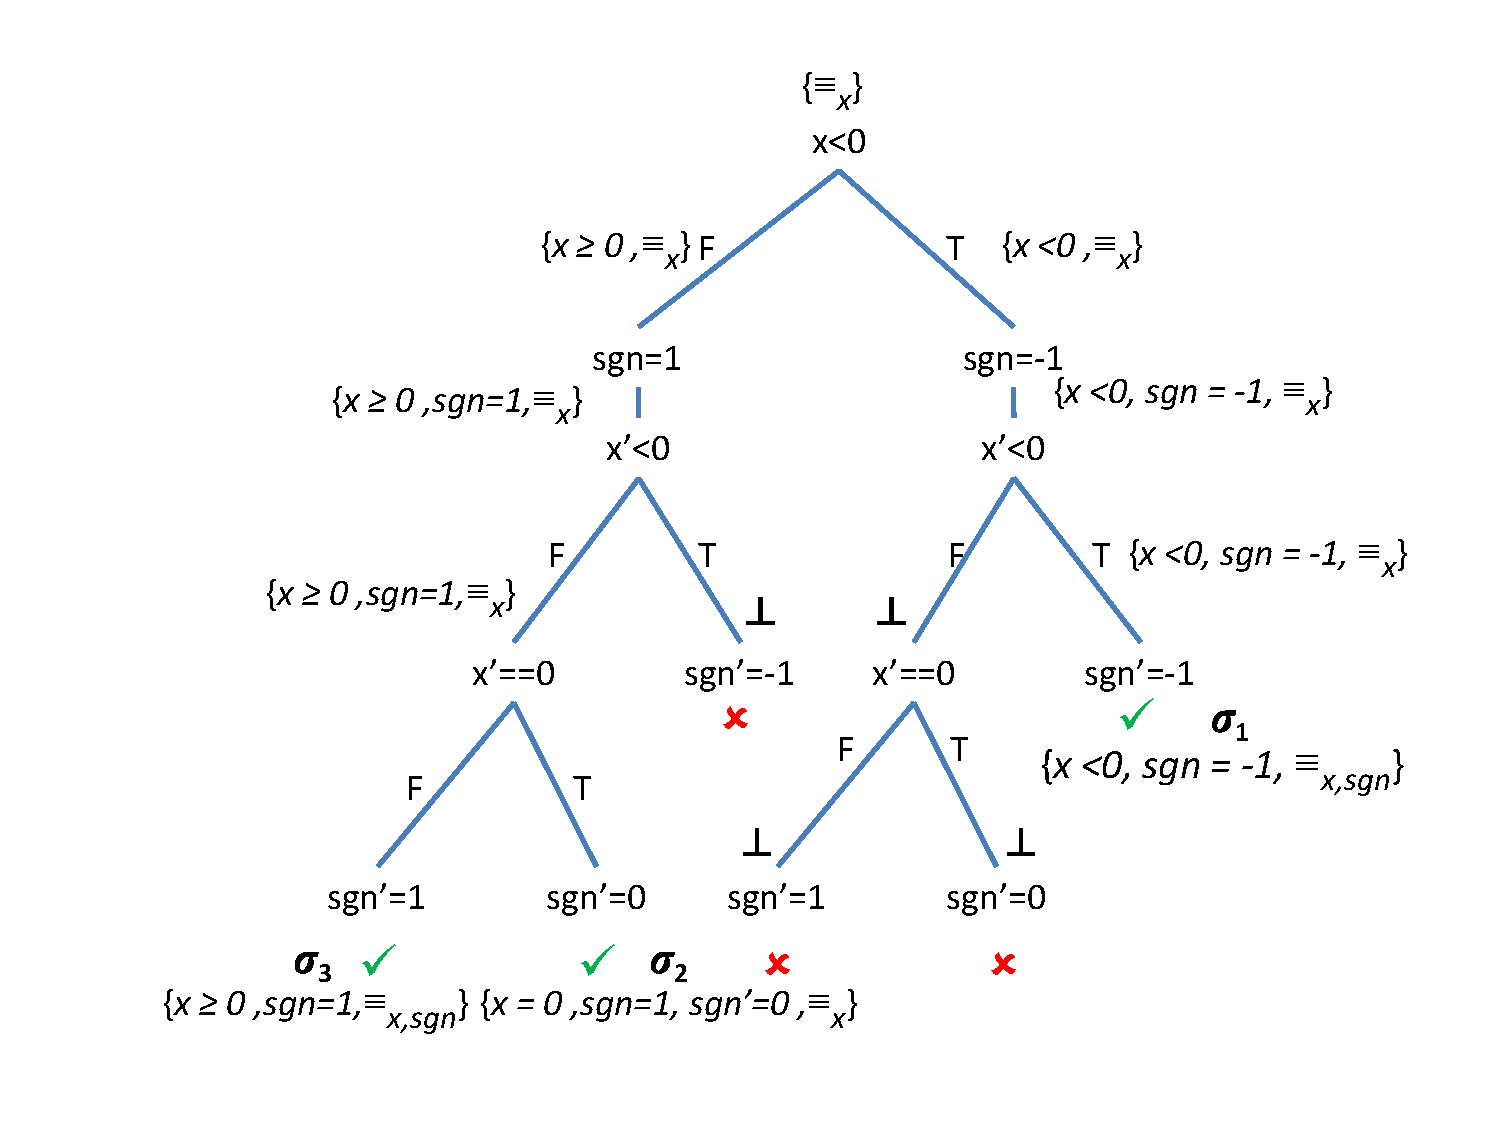
\includegraphics[scale=0.38,clip=true,trim = 75pt 25pt 5pt 20pt]{figures/sign-graph-joint}
\caption{Joint $sign;sign'$ analysis}\figlabel{SignAnalysis1}
\end{figure}

Essentially, our analysis aims to establish correspondence between paths in $P$ and $P'$ by first analyzing all of $P$ paths and then attempting to correlate with $P'$ paths. Clearly, this abstraction is unfeasible for most cases as the number of paths to be considered is exponential (we defer the case of loops where this number is unbound). Therefore we refine our abstraction by using a partially disjunctive domain, partitioned by \emph{equivalence criteria}.

%However, analyzing over $P;P'$ means in the worst case remembering the states along each $P$-path and relating them to states in the corresponding $P'$-path. This approach is similar to the symbolic execution approach~\cite{} where all possible correlating paths are explored individually and output is examined to determine difference whilst attempting to reach full coverage. Much like this approach, this abstraction is unfeasible for most cases, especially for programs with an unbound number of paths e.g. \textbf{loops}. To avoid this we move to a partially disjunctive domain, partitioned by \emph{equivalence criteria}.

As the goal of work is to distinguish equivalent from differencing behaviors, using equivalence as criteria for merging paths is apt. The partitioning will abstract together paths that hold equivalence for the same set of variables, allowing for a maximum of $2^{|VC|}$ disjunctions in the abstract state, where $VC$ is the set of correlated variables. So far we have implicitly defined $VC$ as a correlation between $P,P'$ input and outputs, but our approach is in fact parameterized by this matching, allowing for any $P$ variable to be matched with any of $P'$ which has the potential to provide a more precise result (in the cost of scaling) or alternatively provide a more coarse, scalable result by allowing less variables or only certain equivalence classes of $2^{VC}$. A formal definition and discussion of $VC$ is found in \secref{ConcreteSem}.

For example partitioning the result of \figref{SignAnalysis1} according to our criteria would abstract behaviors $s_1$ and $s_3$ together, as they hold equivalence for $sgn$. The merge would abstract away data regarding $x$ and represent $sgn$ as the $[-1,1]$ interval, losing precision but gaining reduction in state size. This lose of precision is acceptable as it is complemented by the offending state $s_2$. Still, not much is gained from this partitioning, as it is performed at the final state, where we may have already reached an exponential amount of disjunctions.

\begin{figure}
\centering
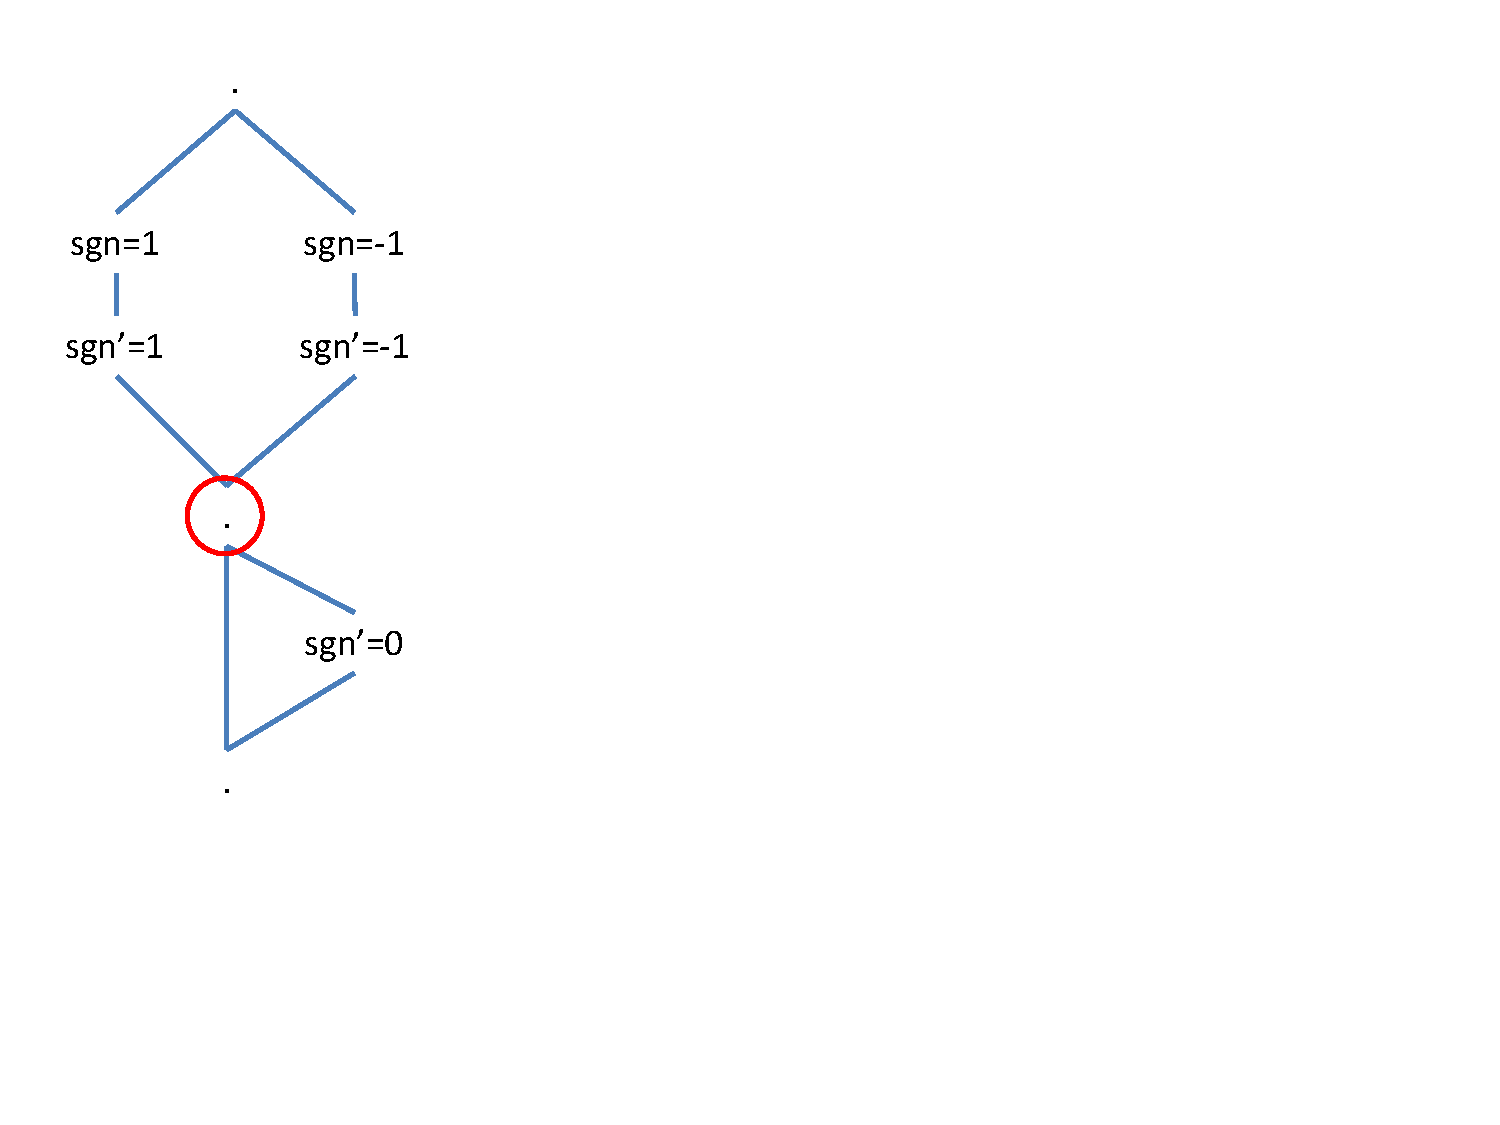
\includegraphics[scale=0.42,clip=true,trim = 0pt 150pt 450pt 150pt]{figures/sign-graph-correlated}
\caption{$sign \bowtie sign'$ analysis}\figlabel{SignAnalysis2}
\end{figure}

To truly gain a reduction of state size, we must perform partitioning dynamically as the analysis is executed i.e. at earlier program locations. This cannot be achieved using a sequential composition $P;P'$. Looking at \figref{SignAnalysis1} we immediately see that equivalence holds only at final states. Intuitively, this is caused due to a command in $P$ having to "wait" for its equivalent command to arrive in $P'$. To overcome this, we present the correlating program $P \bowtie P'$ which allows for earlier partitioning by "saving the need to wait". $P \bowtie P'$ interleaves $P$ and $P'$ commands in an optimized manner, and informs the analysis that it need not wait any further and partitioning is permitted. \figref{SignAnalysis2} depicts the analysis of $sign \bowtie sign'$ (shown in \figref{SignCorrelating}) where the partitioning location is marked with a circle. We define these partitioning locations as \emph{correlation points} (denoted $CP$) and they are a sub product of the correlating program build process. We will further describe the specifics of creating $P \bowtie P'$ in \secref{Correlating} and only shortly say that the interleaving is chosen according to a syntactic diff process over a guarded command language version of the programs.

\begin{figure}
\centering
\begin{lstlisting}
// Nimrod - please fill this 
\end{lstlisting}
\caption{Correlating program $sign \correlate sign'$.}
\figlabel{SignCorrelating}
\end{figure}


% bite the bullet and do widening.
Although we achieved a reduction in state size using partitioning, we have yet to account for programs with an unbound number of paths, created by loops. Unbound path lengths means a potentially unbound analysis as all paths are abstracted. This is mainly where previous approaches fall short ~\cite{GodlinStrichman09, KawaguchiLahiriRebelo10, DwyerElbaumPerson08, EnglerRamos11}. To overcome this, we define a widening operator for our domain, based on the convex sub-domain widening operator. The main challenge here, as our state is a set of convex objects, is finding an optimal pairwise matching between objects for a precise widened result. Optimally, we would like to pair objects that adhere to the same "looping path" meaning we would want to match a path $\pi_i$'s abstraction with a path $\pi_{i+1}$ that results from taking another step in the loop. This basically requires encoding path information along with the sub-state abstraction. This information is acquired by simply keeping guard values explicitly, as they appear in our correlating program, inside the state. As guard values (true or false) reflect branch outcomes, they can be used to match sub-states that advanced on the loop by matching their guard values (for easier matching and better precision we separate guards from other variables in our implementation).

\begin{figure}
\centering
\begin{lstlisting}
int sum(int arr[], unsigned len) {
  int result = 0;
  for (unsigned i = 0; i < len; i++)
    result += arr[i];
 return result;
}
\end{lstlisting}
\caption{A simple looping program for array summation.}
\figlabel{LoopExample}
\end{figure}

We note that the correlating program is cruicial to maintaining equivalence over loops. To demonstrate this we perform the simple exercise of checking equivalence of a small looping program with itself. Consider the array summation program in \figref{LoopExample}. Equivalence for these two small programs cannot be established soundly by approached based on under approximation. To emphasize the importance of the correlating program, we will first show the result of an analysis of $sum;sum'$ which will be:
\\
\begin{tabular}{c}
\hspace{1cm} $\sigma_{\times}^1 = \{len = len' \leq 1, result = result' \mapsto 0\}$
\\
\hspace{1cm} $\sigma_{\times}^2 = \{len = len' > 1\}$
\end{tabular}
\\
\begin{figure}
\centering
\begin{lstlisting}
int sum(int arr[], unsigned len) {
  unsigned len' = len;
  int arr'[] = arr;
  int result = 0;
  int result' = 0;
  {
    unsigned i = 0;
    unsinged i' = 0;
l:  guard g = (i < len);
l': guard g' = (i' < len');
    if (g) result += arr[i];
    if (g') result' += arr'[i'];
    if (g) i++;
    if (g') i'++;
    if (g) goto l;
    if (g') goto l';
  }
}
\end{lstlisting}
\caption{$sum \bowtie sum$}
\figlabel{LoopExample}
\end{figure} 
This lose of equivalence occurred due to the inability precisely track the relationship of $result$ and $result'$ over $sum;sum'$. As we widened the first loop to converge, all paths passing through that loop were merges together, losing the ability to be "matched" with the second loop waiting further down the road. Performing the same analysis on $sum \bowtie sum'$ instead (seen in \figref{LoopCorrelatingExample}), allows maintaining equivalence, as the loops are interleaved correctly to allow establishing $result = result'$ as a loop invariant, surviving the widening process to prove equivalence at the end as the result would be:
\\
\begin{tabular}{c}
\hspace{2cm} $\sigma_{\times}^1 = \{result = result'\}$
\end{tabular}
\\
%The conceptual difference of these two analyses is depicted in \figref{SumWidening}.
%\begin{figure}
%\imagetop{
%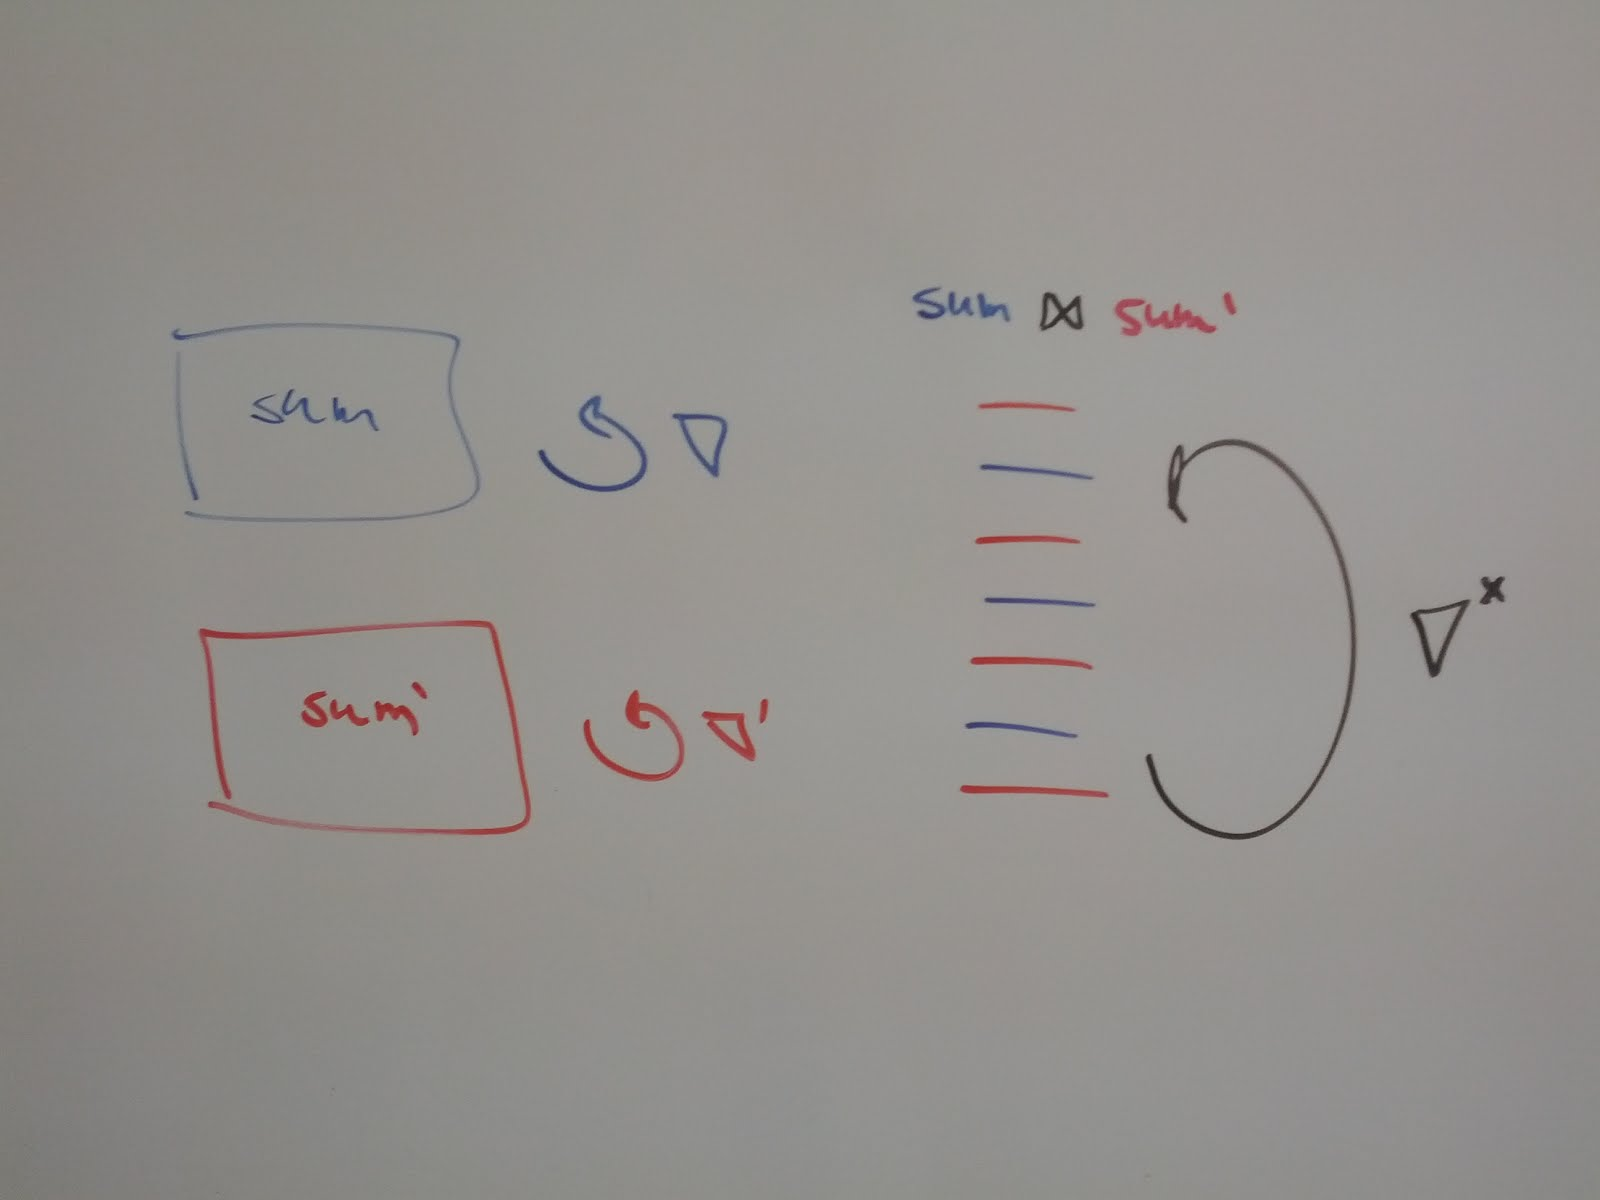
\includegraphics[scale=0.20,clip=true,trim = 150pt 250pt 200pt 200pt]{figures/sum-widening.jpg}
%}
%\caption{Widening $sum ; sum$ vs. $sum \bowtie sum$}\figlabel{SumWidening}
%\end{figure}

\paragraph{Definition of difference}
So far, we defined difference in programs as difference in output variable values at the program final state. Our work extends the notion of difference beyond that, allowing for several program locations to be identified as viable for differentiation (we name these locations \emph{differencing points} denoted $DP$). Other than the programs endpoints, we include every location which:
\begin{itemize}
\item Emits an output value (using a system function or through a global variable)
\item Accesses array
\end{itemize}
This means that procedures may now differ, even if they hold equivalence on the final state. Thus we define difference also as producing a different output value in mid-execution or accessing an array through a different index. This means that programs which differ in array access \emph{patterns} will now be flagged as different. This is a sound approach for difference, as this may include access to illegal bounds (an example for this can be seen in \figref{Md5sumExample}). We note that this definition of description cannot be achieved by instrumenting output or array access through temporary variables and deferring checking their equivalence to the end, as the amount of temporaries needed may be unbound. We therefore require procedures to agree on these locations, in case we wish to verify using the extended definition of difference.
\section{Evaluation of Existing Work}\seclabel{Evaluation}
We have implemented our approach in a tool called {\tool}  based on the \sname{LLVM} compiler infrastructure and the \sname{APRON} numerical abstract domain library, and evaluated our approach on a number of challenging real world programs where the patches affect numerical variables. As benchmarks, we used several programs from the GNU core utilities (differencing versions 6.10 and 6.11), as well as a few handpicked patches taken from the Linux kernel and the Mozilla Firefox web browser. In most programs, we were able to precisely describe the difference.


\subsection{Results}

%% Table generated by Excel2LaTeX from sheet 'Report'
\begin{table*}[htbp]
  \footnotesize
  \centering
  \caption{Experimental Results}
    \begin{tabular}{lrrccccccc}
    \hline
    \textbf{Name} & \textbf{\#LOC} & \textbf{ \#P } & \textbf{Widen} &
        \multicolumn{2}{c}{Interval} &
        \multicolumn{2}{c}{Octagon} &
        \multicolumn{2}{c}{Polyhedra} \\
    &  & &  &
        \textbf{Part} &  \textbf{No Part} &
        \textbf{Part} &  \textbf{No Part} &
        \textbf{Part} &  \textbf{No Part} \\
    \hline
              remove    & 16    & 4     & \xmark     & \xmark(0)        & \xmark(0)         & \checkmark(0:03)  & \checkmark(0:03)  & \checkmark(0:01) & \checkmark(0:01) \\
              copy      & 44    & 2     & \xmark     & \xmark(0:33)     & \xmark(0:33)      & \checkmark(0:23)  & \checkmark(3:11)  & \checkmark(0:07) & \checkmark(0:47) \\
              fmt       & 42    & 5     & \checkmark & \xmark(0:16)     & \xmark(13:20)     & \xmark(3:13)      & $TO$              & \checkmark(0:22) & \checkmark(1:46) \\
              md5sum    & 40    & 3     & \checkmark & \checkmark(0:04) & \checkmark(0:15)  & \checkmark(5:24)  & $TO$              & \checkmark(1:38) & \checkmark(5:52) \\
              pr        & 100   & 10    & \checkmark &                  &                   &                   &                   &                  &                  \\
              savewd    & 86    & 1     & \xmark     & $TO$             & $TO$              & \checkmark(2:53)  & \checkmark(12:37) & \checkmark(0:46) & \checkmark(2:08) \\
              seq       & 23    & 15    & \checkmark & \xmark(0:25)     & \xmark(2:04)      & \xmark(12:21)     & $TO$              & \xmark(3:24)     & \xmark(8:12)     \\
    \hline
              addr      & 77    & 1     & \xmark     & \xmark(0:14)     & \xmark(0:46)      & \checkmark(20:40) & $TO$              & \checkmark(6:46) & $TO$             \\
              nsGDDN    &       & 3     & \xmark     &                  &                   &                   &                   &                  &                  \\
    \hline
              sign      & 8     & 2     & \xmark     & \xmark(0)        & \checkmark(0)     & \checkmark(0)     & \checkmark(0)     & \checkmark(0)    & \checkmark(0)    \\
              sum       & 7     & 5     & \checkmark & \xmark(0:03)     & \xmark(0:10)      & \xmark(0:12)      & \xmark(0:33)      & \checkmark(0:04) & \checkmark(0:14) \\
              nested    &       &       & \checkmark &                  &                   &                   &                   &                  &                  \\
    \end{tabular}
  \tablabel{Results}
\end{table*}

%\tabref{Results} summarizes the results of our analysis. The columns indicate the benchmark name and description, lines of code for the analyzed program, the number of lines added and removed by the patch, the number of diff-points generated, the numerical domain used, and the number of differences found in the analysis (i.e. number of diff-points where $\triangle \neq \varnothing$). In our benchmarks, we focused on computing intra-procedural difference between the two versions of procedures. Procedure calls presented difficulty as they potentially change global variables and local variables through pointers. We overcame this by either (i) assuming equivalence (alone) once we encounter a call to a procedure we already established as equivalent or (ii) warn that all results regarding variables touched by the procedure is un-sound. \TODO{In the majority of our benchmarks we identified calls only to library and system procedures thus we could omit their effect as they do not change variables beyond those given as parameter or those being assigned the return value.} All differences reported describe, in constraints over variables, an existing delta at that program point.

\paragraph{Producing delta from abstract state}

\begin{figure}
\centering
%\begin{tabular}{c}
\begin{lstlisting}
size_t rpc_uaddr2sockaddr (const size_t uaddr_len, ...) {
  char buf[ RPCBIND_MAXUADDRLEN ];
    ...
-  if ( uaddr_len > sizeof ( buf ))
+  if ( uaddr_len > sizeof ( buf ) (*@\textbf{- 2}:@*))
    return 0;
    ...
    (*@\textbf{$(*)_1$}@*)
  buf [ uaddr_len ] = '\n';
  buf [ uaddr_len + 1] = '\0';
    ...
}
\end{lstlisting}
%\\
%Original
%\\
%\hline
%\\
%\begin{lstlisting}
%size_t rpc_uaddr2sockaddr (const size_t uaddr_len, ...) {
%  char buf[ RPCBIND_MAXUADDRLEN ];
%    ...
%  if ( uaddr_len > sizeof ( buf ) (*@\textbf{- 2}:@*))
%    return 0;
%    ...
%    (*@\textbf{$(*)_1$}@*)
%  buf [ uaddr_len ] = '\n';
%  buf [ uaddr_len + 1] = '\0';
%    ...
%}
%\end{lstlisting}
%\\
%Patched
%\end{tabular}
\caption{Linux kernel \scode{addr.c} v2.6.32-rc6 module with patch.}
\figlabel{LinuxExample}
\end{figure} 

\figref{LinuxExample} shows a patch made to the \scode{net/sunrpc/addr.c} module in the Linux kernel \scode{SUNRPC} implementation v2.6.32-rc6 which is aimed at removing an off-by-two array access out of bounds violation in the original program. Although simple, this example shows two advantages {\tool}: (i)~the ability to analyze programs without the need to run them and (ii)~the ability to capture fine-grained differences.\COMMENT{Previous methods would report equivalence for this patch, disregarding the array out of bounds access covered by the patch. Concrete methods~\cite{EnglerRamos11} would require symbolically running the two versions which would be problematic and time consuming considering the size of the system the code is embedded in.} The result of analyzing the correlated program is shown in~\figref{sunrpc}.

\begin{figure}[H]
\scriptsize
\centering
\begin{tabular}{c}
$\sigma_1$:
\\ \hline
returned' = $true$
\\
returned = $false$
\\
uaddr\_len' $\leq$ RPCBIND\_MAXUADDRLEN - 2
\\
uaddr\_len' $\geq$ RPCBIND\_MAXUADDRLEN
\\ \hline
\end{tabular}
\caption{Difference for \scode{rpc\_uaddr2sockaddr}}\label{Fi:sunrpc}

\end{figure}

The difference is captured by one sub-state where the execution has ended in the patched program but continues in the original. We instrument the correlating program with a return flag to capture the difference as otherwise equivalence holds (none of the original variables change).

\paragraph{Capturing complex delta}

\begin{figure}
\begin{tabular}{c}
\begin{lstlisting}
int input_position;

bool char_to_clump(char c) {
  int width;
    ...
+ (*@\textbf{if (width < 0 \&\& input\_position == 0) \{}@*)
+     (*@\textbf{chars = 0;}@*)
+     (*@\textbf{input\_position = 0;}@*)
+ (*@\textbf{\} else if (width < 0 \&\& input\_position <= -width) \{}@*)
+     (*@\textbf{input\_position = 0;}@*)
+ (*@\textbf{\} else \{}@*)
      input_position += width;
+ (*@\textbf{\}}@*)
    (*@\textbf{$(*)_1$}@*)
    ...
  return chars;
}
\end{lstlisting}
\end{tabular}
\caption{Original and patched version of coreutils \scode{pr.c}'s \scode{char\_to\_clump} procedure}
\figlabel{PrExample}
\end{figure} 

\figref{PrExample} shows a patch made to the \scode{char\_to\_clump} function in version 6.11 of coreutils. The patch replacing the execution of the line \scode{input\_position += width}, which originally executed unconditionally, with a conditional structure that in the new version, allows the line to execute only under certain complex conditions. Since the variables handled in this patch (the global \scode{input\_position} and return value \scode{chars}) emit output, describing how their values changed and under which terms is important, especially as the patch cannot be easily parsed by a programmer to understand its meaning. The result of our analysis at the return point is show in \figref{CharToClump}. These results include information regarding initial values of parameters for improved precision.

\begin{figure}[H]
\scriptsize
\centering
\begin{tabular}{l|l|l}
$\sigma_1$:                 & $\sigma_2$:                   & $\sigma_3$:
\\ \hline
input\_position${_0}$ = 0     & input\_position${_0}$  < -width & input\_position${_0}$  < -width
\\
chars' = 0                & input\_position${_0}$  < 0      & input\_position${_0}$  > 0
\\
input\_position = width   & input\_position' = 0        & input\_position' = 0
\\
input\_position < 0       & input\_position < width     & input\_position > width
\\
input\_position' = 0      & width < 0                   & input\_position <= 0
\\ \hline
\end{tabular}
\caption{Difference for coreutils pr.c \scode{char\_to\_clump}}\label{Fi:CharToClump}
\end{figure}


The result convey the difference in the output variable values alongside some of conditions under which the difference occurs. The result is composed of three sub-states featuring difference and adhere to two added paths in the patched program. The first sub-state belongs to the first branch in the added conditional: the difference is comprised of (i) the new value of \scode{input\_position} is 0 as opposed to it being \scode{width} in the former version (the analysis took the \scode{input\_position += width} line into account and incorporated knowing that $input\_position = 0$ from the branch condition). The analysis also deduced that the old \scode{input\_position} is negative under the same input as the branch condition dictates that \scode{width} is negative. (ii) \scode{chars} in the new program is 0 under this path. The two other sub-states adhere to the second added path in the conditional and track a difference for \scode{input\_position} alone, basically stating that \scode{input\_position} under this path used to assume values in ranges $[-\inf,width]$ and $[width,0]$ but now is simply 0. The splitting of this path into two cases is a result of expressing the non-convex $input\_position \neq 0$ condition from the first branch conditional using two sub-states. The result also describes constraints on the procedure's input under which the difference exist. Another product of the analysis, which we do not show here, are sub-states describing paths which the patch did not affect.

\paragraph{Maintaining Equivalence and Reporting Difference in Loops}

\begin{figure}[H]
\centering
%\begin{tabular}{cc}
\begin{lstlisting}
bool bsd_split_3 (char *s, size_t s_len,...) {
  int i = s_len;
  i--;
+ (*@\textbf{if (s\_len == 0) return false;} @*)
  while (i && s[i] != ')') { (*@\textbf{$(*)_1$} @*)
    i--;
  }
  ...
  (*@\textbf{$(*)_2$} @*)
}
\end{lstlisting}
%&
%\begin{lstlisting}
%bool bsd_split_3 (char *s, size_t s_len,...) {
%  int i = s_len;
%  i--;
%
%  i = s_len - 1;
%  while (i && s[i] != ')') { (*@\textbf{$(*)_1$} @*)
%    i--;
%  }
%  ...
%  (*@\textbf{$(*)_2$} @*)
%}
%\end{lstlisting}
%\\
%coreutils md5sum.c v6.10 & coreutils md5sum.c v6.11
%\end{tabular}
\caption{Original and patched version of coreutils \scode{md5sum.c}'s \scode{bsd\_split\_3} procedure}
\figlabel{Md5sumExample}
\end{figure} 
We explore a challenging loop scenario where all paths in the programs contain loops and only some of them maintain equivalence. \figref{Md5sumExample} shows part of coreutils md5sum.c \scode{bsd\_split\_3} function that was patched in version version 6.11 to disallow 0-length inputs. Although this patch seems trivial, analyzing it is challenging as it affects the behavior of loops i.e. unbound path lengths. The main challenge in this example, is separating the path where $s\_len$ is 0, which results in the loop index $i$ ranging within negative values (producing an array access out of bounds fault), from the rest of the behaviors that maintain equivalence, throughout the widening process which is required for the analysis to reach a fixed point. The result of our analysis with partitioning is shown in \figref{bsdSplit}~(a) (per differencing points $(*)_{1},(*)_{2}$).

\begin{figure}[H]
\scriptsize
\centering
\begin{tabular}{c}
\begin{tabular}{l||l}
\begin{tabular}{l|l}
\multicolumn{2}{l}{$(*)_1$:}
\\ \hline
$\sigma_1$:     & $\sigma_2$ (equivalent):
\\ \hline
s\_len = 0      & s\_len' = s\_len
\\
s\_len' = 0     & i' = i
\\
i $\leq$ -1     & s\_len' - 1 $\geq$ i'
\\ \hline
\end{tabular}
&
\begin{tabular}{l}
\multicolumn{1}{l}{$(*)_2$:}
\\ \hline
$\sigma_1$ (equivalent):
\\ \hline
s\_len' = s\_len
\\
i' = i
\\
s\_len' - 1 $\geq$ i'
\\ \hline
\end{tabular}
\end{tabular}
\\ \\ (a) \\
\begin{tabular}{l||l}
\begin{tabular}{l|l|l}
\multicolumn{2}{l}{$(*)_1$:}
\\ \hline
$\sigma_1$:     & $\sigma_2$ (equivalent):  & $\sigma_3$ (equivalent):
\\ \hline
s\_len = 0      & s\_len' = s\_len          & s\_len' = s\_len
\\
s\_len' = 0     & i' = i                    & i = 0
\\
i $\leq$ -1     & s\_len' - 1 $\geq$ i'     & s\_len' $\geq$ 1
\\ \hline
\end{tabular}
&
\begin{tabular}{l}
\multicolumn{1}{l}{$(*)_2$:}
\\ \hline
$\sigma_1$ (equivalent):
\\ \hline
s\_len' = s\_len
\\
i' = i
\\
i = 0
\\
s\_len' $\geq$ 1
\\ \hline
\end{tabular}
\end{tabular}
\\ \\ (b)
\end{tabular}
\caption{Difference for \scode{bsd\_split\_3}}\label{Fi:bsdSplit}
\end{figure}

We can see the analysis successfully reports a difference for the singularity point $s\_len = 0$ inside the loop, precisely describing the scenario where $i'$ is negative. We can also see the other equivalent state existing within the loop which depicts the results of the widened analysis for all other paths (the $s\_len \neq 0$ constraint is not existing there due to partitioning as we will soon show). The differencing sub-state will be omitted once we move past the loop as the $i \leq -1$ constraint will not allow it to exist beyond the loop body \COMMENT{(we do not account for overflow at this point in our work as ???)} thus we are left with the equivalent state alone after the loop which correctly expresses the fact that the programs are equivalent at this point (since both i's converged at 0). We can see that the result at the second differencing point has lost precision since it does not reflect the $i = 0$ constraint. The loss of this constraint is, again, due to partitioning as both sub-states that describe exiting the loop and the one describing entering the loop, hold equivalence for all variables and are joined to together and lose the extra constraint information.
\COMMENT{? describe the canonization for the example}
If we analyze the same example with no partitioning we get the result of \figref{bsdSplit}~(b).

Which further separates the paths in the program, allowing for a different sub-state for the $i = 0$ and $i \neq 0$ substates (again, the $i \neq 0$ constraints was lost when joining together the $i > 0$ and $i < 0$ states as they both adhere to the same path and hold the same guard values). This extra precision is beneficial, but we still managed to supply a satisfactory result using the more scalable partitioning by equivalence technique.

%% Table generated by Excel2LaTeX from sheet 'Report'
\begin{table*}[htbp]
  \footnotesize
  \centering
  \caption{Experimental Results}
    \begin{tabular}{lrrccccccc}
    \hline
    \textbf{Name} & \textbf{\#LOC} & \textbf{ \#P } & \textbf{Widen} &
        \multicolumn{2}{c}{Interval} &
        \multicolumn{2}{c}{Octagon} &
        \multicolumn{2}{c}{Polyhedra} \\
    &  & &  &
        \textbf{Part} &  \textbf{No Part} &
        \textbf{Part} &  \textbf{No Part} &
        \textbf{Part} &  \textbf{No Part} \\
    \hline
              remove    & 16    & 4     & \xmark     & \xmark(0)        & \xmark(0)         & \checkmark(0:03)  & \checkmark(0:03)  & \checkmark(0:01) & \checkmark(0:01) \\
              copy      & 44    & 2     & \xmark     & \xmark(0:33)     & \xmark(0:33)      & \checkmark(0:23)  & \checkmark(3:11)  & \checkmark(0:07) & \checkmark(0:47) \\
              fmt       & 42    & 5     & \checkmark & \xmark(0:16)     & \xmark(13:20)     & \xmark(3:13)      & $TO$              & \checkmark(0:22) & \checkmark(1:46) \\
              md5sum    & 40    & 3     & \checkmark & \checkmark(0:04) & \checkmark(0:15)  & \checkmark(5:24)  & $TO$              & \checkmark(1:38) & \checkmark(5:52) \\
              pr        & 100   & 10    & \checkmark &                  &                   &                   &                   &                  &                  \\
              savewd    & 86    & 1     & \xmark     & $TO$             & $TO$              & \checkmark(2:53)  & \checkmark(12:37) & \checkmark(0:46) & \checkmark(2:08) \\
              seq       & 23    & 15    & \checkmark & \xmark(0:25)     & \xmark(2:04)      & \xmark(12:21)     & $TO$              & \xmark(3:24)     & \xmark(8:12)     \\
    \hline
              addr      & 77    & 1     & \xmark     & \xmark(0:14)     & \xmark(0:46)      & \checkmark(20:40) & $TO$              & \checkmark(6:46) & $TO$             \\
              nsGDDN    &       & 3     & \xmark     &                  &                   &                   &                   &                  &                  \\
    \hline
              sign      & 8     & 2     & \xmark     & \xmark(0)        & \checkmark(0)     & \checkmark(0)     & \checkmark(0)     & \checkmark(0)    & \checkmark(0)    \\
              sum       & 7     & 5     & \checkmark & \xmark(0:03)     & \xmark(0:10)      & \xmark(0:12)      & \xmark(0:33)      & \checkmark(0:04) & \checkmark(0:14) \\
              nested    &       &       & \checkmark &                  &                   &                   &                   &                  &                  \\
    \end{tabular}
  \tablabel{Results}
\end{table*}



\section{Related Work} \seclabel{Related}

Our work has been mainly inspired by recent work identifying program differencing as having vast security implications~\cite{BrumleyPoosankamSongZheng08,SongSunZhang09} as well as advancements made in the field of under-approximations of program equivalence~\cite{GodlinStrichman09, KawaguchiLahiriRebelo10, DwyerElbaumPerson08, EnglerRamos11}.

The problem of program differencing is fundamental~\cite{Hoare69} and early work mainly focused on computing syntactical difference~\cite{HuntMcIlroy75}. These solutions are an important stepping stone and we used syntactical diff as a means to achieve interleaving of programs in out correlating program for better analysis results. Another possibility for creating this program is to rely on the editing sequence that creates the new version from the original program~\cite{Horwitz90}.

Jackson and Ladd~\cite{JacksonLadd94} proposed a tool for computing data dependencies between input and output variables and comparing these dependencies along versions of a program for discovering difference. This method may falsely report difference as semantic difference may occur even if data dependencies have not changed. Furthermore, data dependencies offer little insight as to the meaning of difference i.e. input and output values. Nevertheless, this was an important first step in employing program analysis as a means for semantic differencing.

Several works on the problem of equivalence of combinatorial circuits~\cite{KuehlmannKrohm97,BraytonChatterjeeMishchenkoEen06, ClarkeKroening03} made important contributions in establishing the problem of equivalence as feasible, producing practical solutions for hardware verification.

We rely on classic methods of abstract interpretation~\cite{CousotCousot77} for presenting an over approximating solution for semantic differencing and equivalence. To achieve this we devised a static analysis over a correlating program. The idea of a correlating program is similar to that of self-composition~\cite{AikenTerauchi05} except that we compose two different programs in a interleaving designed to maintain a close correlation between them. The use of a correlating construct for differencing is novel as previous methods mainly use sequential composition~\cite{GodlinStrichman09, DwyerElbaumPerson08, EnglerRamos11}, disregarding possible program correlation.

We base our analysis on numerical abstractions~\cite{CousotHalbwachs78, Mine2006} that allow us to reason about variables of different programs. The abstraction is further refined in a way similar to trace partitioning~\cite{MauborgneRival07} with an equivalence-based partitioning criteria.

Symbolic execution based methods~\cite{DwyerElbaumPerson08, EnglerRamos11} offer practical equivalence verification techniques for loop and recursion free programs with small state space. These works complement each other in regards to reporting difference as one ~\cite{DwyerElbaumPerson08} presents an over approximating description of difference they call differential summaries and the other~\cite{EnglerRamos11} presents an under approximating description including concrete inputs for test cases demonstrating difference in behavior. An interesting question is how could these methods be combined iteratively to achieve better precision. Also, this work can be used to complement our work in cases where equivalence could not be proven and the description of difference can be leveraged for the extraction of concrete input that leads to offending states.

Bounded model checking based work~\cite{GodlinStrichman09} presents the notion of partial equivalence which allows checking for equivalence under specific conditions, supplied by the user but are bound by loops. They employ a technique based on theorem provers for proving an equivalence formula which embeds program logic (in SSA form) alongside the requirement for input and output equivalence and user provided constraints.

\cite{AmitRinetzkyRepsSagivYahav07} introduced a correlating heap semantics for verifying linearizability of concurrent programs. In their work, a correlating heap semantics is used to establish correspondence between a concurrent program and a sequential version of the program at specific linearization points.  
%\section{Research Uniqueness}\seclabel{Uniqueness}

As our work addresses a hot topic where much work is being done, we emphasize here the methods and ideas that differentiate our work from those of others:

\begin{itemize}
\item The use of a correlating program which allows of a joint analysis of two versions of a program \textbf{at each program point} allows for a more precise and scalable analysis. Other techniques compare only final states of the programs thus missing key differences in mid-execution that effect program behavior. Also, comparing final states in less scalable.
\item Analysis using a correlating domain is superior to separate analysis. Any separate two program states (belonging to two program versions) can be soundly and more precisely represented by one joint state which can hold data of equivalence between versions of variables, as well as standard state data (held by the two separate states). This is because \textbf{equivalence under abstraction does not imply concrete equivalence}.
\item Our non-convex domain allows us to report non-convex differences -- a more precise result than those achieved by standard domains. As other will report that some, unknown, difference is possible, we are able to better characterize the difference while maintaining scalability.
\item We developed a differential analysis framework for C programs based on the open source LLVM compiler infrastructure. We have not witnessed any other research that supplies such an extensive open source tool.
\end{itemize} 
\section{Future Work}\seclabel{Future}

In this section we will first outline the different aspects of the differential analysis problem and discuss questions and research directions which derive from them. Second, we will propose a time line for exploring these directions throughout the research. As the problem of differential analysis is vast, we do not plan to explore all proposed directions immediately (some will not appear in the research plan and will be considered as the research progresses).

\subsection{Problem Dimensions}

We first describe a brief overview of the problem dimensions and later elaborate on each of the proposed directions:

\para{Program Correlation}
\begin{itemize}
\item Limitations of current correlating technique.
\item Static construction of correlating program - explore other methods for producing the correlating program e.g. using control flow graphs.
\item Dynamically (during analysis) creating program correlation, according to analysis data.
\end{itemize}

\para{Definition of Difference}
\begin{itemize}
\item Extending the notion of difference beyond output equivalence.
\item Examining how patching a program affects it safety specification (i.e. assertions).
\end{itemize}

\para{Extending Analysis Domain}
\begin{itemize}
\item Performing inter-procedural analysis using function summaries.
\item Detecting difference in float, pointer and heap data types.
\item Analyzing binary code.
\end{itemize}

\para{Other Analysis Techniques}
\begin{itemize}
\item Using static results for directing symbolic execution to find differencing inputs.
\item Using concolic execution to find differencing inputs.
\end{itemize}


\subsubsection{Program Correlation}

The problem of correlating executions of different programs for differentiation is only partially addressed in our work so far. We chose to use a standard semantics over a correlating program in order to leverage existing analysis techniques (that were adapted to maintain information about variable correlations). We constructed our correlating program using a simple syntactic diff algorithm over imperative commands of normalized programs. This method performs well on many examples, but may still produce a result that defies successful analysis, when encountered with complex language features or more drastic program changes.
\COMMENT{
\paragraph{Guarded Commands Format}
The process of creating a correlating program entails the transformation of C programs into a guarded command format s.t. programs may be interleaved correctly. This process is not trivial and must be carefully executed to preserve semantics. As there exists no production grade tool that performs this C-to-C transformation, it was implemented as a part of the research. However, this transformation is not yet complete as it does not handle all of the complex C program features. Since this transformation can be useful for various applications (it allows program interleaving), and specifically our research, we consider further extending and completing it towards using it as a building block for other research.
}

\paragraph{Correlating Program Caveats}
A more careful examination of the correlating program, reveals that branching may break program semantics. By observing any of the correlating programs examples that contain a branching \scode{goto} command, one sees that if the branch destination of one program conflicts with that of the second program, the second program semantics will change (and vice versa). This has not been a problem for the set of examples we handled so far, since every branch in one program was immediately followed by a branch in the other - to the same destination. However, this needs adjustment if we strive to handle more complex, larger examples. Correct composition of programs requires instrumenting the programs with an explicit program counter, and executing instructions according to the value of the counter. This can produce a more dynamic composition that allows more control over which program advances at each step. An example of such composition for the program from \figref{SignExample} is shown in \figref{SignCorrelating2}.

\begin{figure}[H]
\centering
\begin{tabular}{c}
\begin{lstlisting}
int sign(int x) {
  int x' = x;
  int pc = 0, pc' = 0;
  int turn = 1;
  while (pc < 3 || pc' < 5) {
  if (turn) {
      switch (pc) {
        case 0: guard g1 = (x < 0); pc++;   turn = 0;   break;
        case 1: if (g1) sgn = -1;   pc++;   turn = 0;   break;
        case 2: if (!g1) sgn = 1;   pc++;   turn = 0;   break;
        default:                            turn = 0;   break;
      }
  } else {
      switch (pc') {
        case 0: guard g1' = (x' < 0);   pc'++;   turn = 1;   break;
        case 1: if (g1') sgn' = -1;     pc'++;   turn = 1;   break;
        case 2: if (!g1') sgn' = 1;     pc'++;   turn = 1;   break;
        case 3: guard g2' = (x' == 0);  pc'++;               break;
        case 4: if (g2') sgn' = 0;      pc'++;               break;
        default:                                             break;
      }
  }
}
\end{lstlisting}
\end{tabular}
\caption{Correlating program $sign \correlate^* sign'$ according to the new format.}
\figlabel{SignCorrelating2}
\end{figure} 

The program counters are instrumented as the variables $pc$ and $pc'$. The variable $turn$ is used to determine which of the programs will advance next. This decision can be altered during the analysis process to advance further over one program, this can also be determined dynamically (for dynamic analysis methods).

\paragraph{Program Graph Correlation}
Our method for composing programs so far has used the textual representation sequential order of commands as a basis for composition. We took the vectors of (guarded) commands from both programs and tried to match it using a syntactic diff. However, there is much potential in applying other techniques for finding this matching. Previous work addressing syntactical methods for program equivalence using graph representation~\cite{Horwitz89,Horwitz90} can be used to find a matching for differentiation. This matching, unlike ours, considers all sort of instructions in the program (i.e. branch conditionals, etc. as well as imperative commands).

\paragraph{Correlation Refinement} The correlating program is an input for the analysis process and effectively determines the order in which each of the programs will execute alternately. We raise the question: does this ``scheduling'' need be predetermined? The analysis can defy the constant interleaving supplied by the correlating program and choose to execute more commands of one program instead of alternating to the other program to try and explore a better result. The immediate criteria for defining this ``better'' result would be equivalence, i.e. the analysis would choose to advance further in the execution of one program, until it reached a more equivalent abstract state (where more variables maintain equivalence). An example where such a techniques is useful can be seen in \figref{SeqExample}.

\begin{figure}[H]
\centering
\begin{tabular}{c}
\begin{lstlisting}
static void
print_numbers (long first, long step, long last, ...)
{
  long i;
  for (i = 0; /* empty */; i++) {
    long x = first + i * step;
    if (step < 0 ? x < last : last < x) break;
    if (i) fputs (separator, stdout);
    printf (fmt, x);
  }
  if (i)
    fputs (terminator, stdout);
}
\end{lstlisting}\\
coreutils seq.c v6.9 \\
\hline
\\
\begin{lstlisting}
static void
print_numbers (long first, long step, long last, ...)
{
  bool out_of_range = (step < 0 ? first < last : last < first);
  if (! out_of_range) {
    long x = first;
    long i;
    for (i = 1; /* empty */ ; i++) {
      printf (fmt, x);
      if (out_of_range) break;
      x = first + i * step;
      out_of_range = (step < 0 ? x < last : last < x);
      if (out_of_range){
        bool print_extra_number = false;
        ... // print_extra_number is decided here
        if (! print_extra_number) break;
      }
      fputs (separator, stdout);
      }
    fputs (terminator, stdout);
  }
}
\end{lstlisting}
\\
coreutils seq.c v6.10
\end{tabular}
\caption{Original and patched version of coreutils \scode{seq.c}'s \scode{print\_numbers} procedure}
\figlabel{SeqExample}
\end{figure} 

Trying to find a textual correlation between these two version will produce poor results, and existing approaches will not be able to capture the fact that these versions only differ slightly, since only one extra output will be emitted (for the case where $out\_of\_range$ is true and $print\_extra\_number$ is true). In this example, if we allow the analysis to choose the order of alternation between programs, until it reaches a point of output (where it can be established that $x$ is equivalent in both versions), it will produce a result stating that the programs are equivalent up to the point where the extra number is printed. This examples shows an ``equivalence-in-output'' advancement criteria where the analysis will advance on both programs until it reaches a point that emits output, and only then check for difference.

We name this technique ``equivalence-guided correlation refinement''.

\subsubsection{Definition of Difference}

\paragraph{Extending the Notion of Difference}
Previous work regarding semantic differencing~\cite{DwyerElbaumPerson08, GodlinStrichman09, EnglerRamos11, HawblitzelKawaguchiLahiriRebelo12} define program difference as difference between outputs in final state. This notion of difference may be insufficient, as observable behavioral changes may appear before the program terminates (as explained in \secref{OverviewDiffDef}. We explore extending the notion of difference towards (i) array access indexes (ii) output functions (iii) assertion violations. This means that our analysis will compute difference at these locations - specifically for variables which values affect access index, output value and assertion correctness - as well as the final state. This task is not trivial for all programs, as different program versions can emit a difference number of output, or access different arrays. These scenarios require further study.

\paragraph{Specification Guided Differential Analysis}
Proposing to compute program difference at assertion locations introduces safety specifications into the domain of differential analysis. One may wish to ignore output equivalence and concentrate on the question of \emph{how does patching a certain program affect its safety specification}? (as reflected by assertions). This has the potential to be a simpler problem and a lower hanging fruit as we have seen no previous work addressing this particular question. One can further leverage the program specification, by assuming it as part of the analysis process for a sort of ``delta verification'' technique which relies on the hypothesis that the previous version holds up to its specification, and tries to verify that the patched version does so as well. For programs that lack specifications, memory safety specifications can be automatically generated based on previous work~\cite{ConditHarrenMcPeakNeculaWeimer03}.


\subsubsection{Extending Analysis Domain}\seclabel{ExtendedAnalysis}

So far we have explored using only intra-procedural static analysis over a correlated program with numerical abstract domains. This can be vastly extended as follows:

\paragraph{Dual Program Analysis}
As mentioned, performing the analysis over the correlating program has disadvantages as it requires a complex canonization and composition of programs. We consider porting our analysis framework to work over two program CFGs. This will alleviate the need for performing complex transformation and composition and will also allow us to implement correlation refinement as we can independently choose on which of the program graphs we wish to advance (conceptually, this could also be performed on the correlated program but with much less ease). This will also allow us to easily use graph correlation techniques for choosing the order of advancement over the two programs. The disadvantage of this method is that it does not create a single, runnable correlating program (that can by used by other techniques as described in \seclabel{OtherAnalysis}).

\paragraph{Inter-procedural Analysis}
We aim to achieve a better inter-procedural analysis technique as we now rely on modular analysis of function calls to prove equivalence or inlining in case equivalence cannot be proven. Specifically, we plan to explore the use of procedure summaries~\cite{RepsHorwitzSagiv95} over correlating programs.

\paragraph{Floats, Pointers, Arrays and Heap Domains}
Existing differential analysis techniques fall with respect to floats, arrays, and heap-allocated data structures, as symbolic execution mainly applies to integer variables. In the first step, we plan to enrich our abstract representation using aliasing information obtained by simple points-to analysis~\cite{Steensgaard96,Andersen94}. As a second step, we will consider combination with shape analysis~\cite{SagivRepsWilhelm02}.

\COMMENT{
\paragraph{Analyzing Concurrent Programs}
}

\paragraph{Binary Analysis}
An exciting application of differential analysis is automatic generation of exploits from patches. This is most relevant in the setting of binary code as security implications are most significant for programs that are usually released in binary form as an attempt to achieve ``security by obscurity'' (e.g. operating systems libraries, browsers). Previous work in generating exploits from patches for binaries~\cite{BrumleyPoosankamSongZheng08} operated by first locating added input sanitation checks in the patched binary and then producing input that fails these checks by computing the weakest precondition for failing the check. Next, dynamic (examining program executions) and static (analyzing program CFG) techniques were employed to find a path in the program that leads to a state satisfying the aforementioned weakest precondition. This method generated impressive results and found several security flaws in libraries of the Windows operating system. This method can be further extended by performing a comprehensive analysis for finding all program differences, including those that are not captured by added sanitation checks. Such an analysis allows generation of more exploits, for instance those that are no trivially fixed by a sanitation check or those that are \emph{accidently added} by the patched program. Furthermore, this analysis can be useful for legacy or external code where the source is not available. Efficiently differencing legacy code from new code is perhaps the most desirable application of differential analysis. To achieve this we plan to modify our analysis to operate over the LLVM intermediate representation language~\cite{LattnerAdve04}. This intermediate language is high-level enough to support program analysis, and mature enough as it contains static analysis facilities for numerous existing analyses. Most importantly, LLVM-IR has several translations from various languages, including a project~\cite{Scheller:2009} for translating all QEMU~\cite{Bellard05} supported machine code (including x86, ARM, etc.). This can also allow finding exploits for non standard devices such as handhold devices (iOS, Android) - a direction yet to be explored.

\subsubsection{Other Analysis Techniques}\seclabel{OtherAnalysis}
We do not limit ourselves purely to static methods and abstract interpretation. The experience and techniques gained in our research so far can be used to apply other analysis techniques successfully.

\COMMENT{
\paragraph{Dynamic Analysis.} We plan to employ dynamic analysis techniques, for finding differences by running both versions of the program with the same input and check for equivalence between output states. This method is lacking as it is not able to detect differences that occur during execution such as array accesses, pointer de-referencing etc. Using our \emph{correlating program} however, we can detect these differences as we can compare values at differencing points.
}
\paragraph{Statically Directed Symbolic Execution.} This method has become very popular in achieving better test coverage for programs~\cite{GodefroidKlarlundSen05} and recent work in the field of differential analysis has employed this method for comparing program versions~\cite{DwyerElbaumPerson08}. Although this method is not sound, it offers results with zero false positives. The general algorithm performed by these works is as follows: Given a pair of procedures $(P,P')$ symbolically execute the programs with symbolic inputs $(i,i')$ to collect path constraints on $P$ (denoted $C_{\pi}$) first and then $P'$ (denoted $C'_{\pi'}$). Some effort is made to direct the symbolic execution towards locations where \emph{textual difference} is found. Eventually, an SMT solver is used to find a solution for the formula: $i = i' \wedge C_{\pi} \wedge C'_{\pi'} \wedge retval \neq retval'$. If a solution is found for said constraint then a differncing input is found, otherwise, the algorithm continues by trying to negate one of the branches in the previously selected paths and proceed to symbolically execute from there, or try to direct the execution towards a new location that contains textual difference. We wish to improve on this method by using the results of our preliminary analysis to achieve better coverage. Our analysis produces an abstract state describing difference at a certain program point. This can be leveraged to (i) direct the symbolic execution towards locations with symbolic difference, this is superior to current syntactic difference (ii) extract constraints from the abstract state to reduce the search space for the decision procedure. \COMMENT{We performed a preliminary experiment, using the KLEE symbolic execution engine~\cite{CadarDunbarEngler08} to run a few of our correlated programs.}

\paragraph{Statically Directed Concolic Execution.} A method combining testing (\textbf{conc}rete) and symbolic execution (symb\textbf{olic}) which is more scalable as only part of the execution is symbolically represented and the rest runs with concrete values~\cite{ChipounovKuznetsovCandea12} thus we conceptually cover several paths in the same execution. The use of concrete values also overcomes complex program operations and may replace function calls that encumber the underlying SMT solver. We consider experimenting with the $S^{2}E$ ~\cite{ChipounovKuznetsovCandea12} advanced concolic execution engine for exploration of all paths containing difference, based on previous data collected using our static method (which will direct us to differencing program locations). We note that this approach (even without the preliminary static state) has not been researched by previous work.


\subsubsection{Future Evaluation}

Finally we will discuss the method we plan on evaluating our work with.
\begin{enumerate}
\item \textbf{Synthetic Challenge Programs}: We will test on a set of short program, each presenting a different challenge for differential analysis, including: variable and location correlation, false differences, false equivalence, loops, etc. to evaluate the advantages and pitfalls of each technique.
\item \textbf{GNU Coreutils}: We will test on the coreutils benchmark of medium length C programs. These will give us a clue as to how we perform on real world code.
\item \textbf{Patch Survey}: We will perform a survey of patching to determine how patches look in large scale programs (OS, browsers, etc.) and which features they include and evaluate how our tool will perform there.
\end{enumerate}

\COMMENT{
\subsubsection{Applications}

\begin{enumerate}
\item \textbf{Producing Differencing Inputs}
\end{enumerate}
}

\subsection{Research Timeline}
The following are the immediate research topics we plan to address. We will consider other topics as mentioned in \secref{Intro} as our research advances and according to the results of our immediate plans.

\begin{enumerate}
\item Improve our existing tool to achieve compelling results on a larger set of real numerical programs. Our tool will be able to process large code examples and produce a precise and useful delta when such exists or prove no delta exists. -- 2 months.
\item Explore interaction between the structure of the correlating program and the abstractions required to precisely capture program differences. Also explore the creation of a correlating program vs. dual-program analysis.
\item Explore applying dynamic analysis methods such as fuzz testing, concolic and symbolic execution to correlating programs in order to evaluate how these methods perform and scale in regards to our static approach as well as extract differentiating input towards test case generation applications -- 8 months.
\item Combine static and dynamic analysis methods to obtain better precision and extracting more differencing program input for automatic test case generation. Use static analysis directed symbolic execution for maximum scalability and precision -- 6 months
\COMMENT{
\item Extend our tool to run on array and pointer programs -- 5 months.
\item Explore correlation refinement guideless analysis for achieving better precision. -- 4 months.
}
\end{enumerate}



\bibliographystyle{acm-nice}
\newpage
\bibliography{bib}

\newpage
\appendix

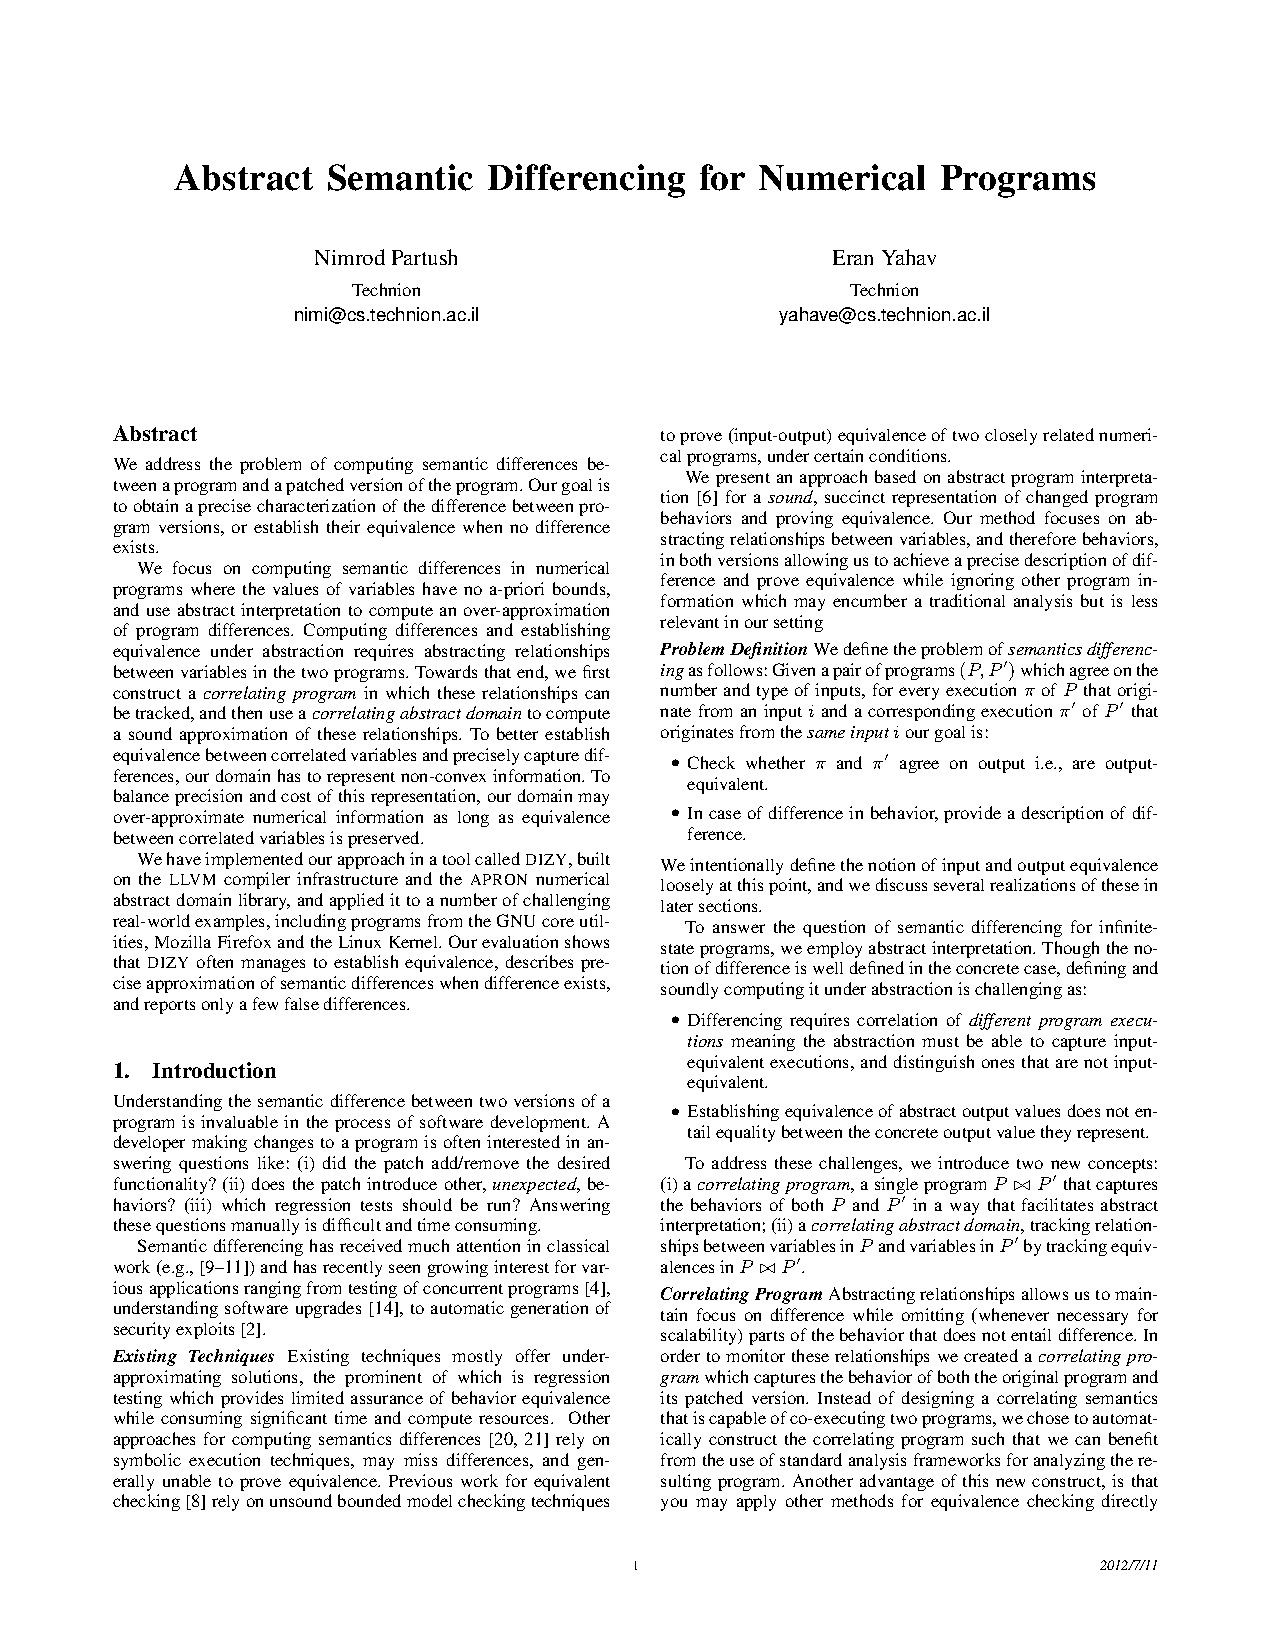
\includepdf[pages={1-12}]{paper.pdf}

\end{document}
